\documentclass[preprint,12pt,authoryear]{elsarticle}
\usepackage[utf8]{inputenc}
\usepackage[T1]{fontenc}
\usepackage{amsmath,amssymb,amsfonts,bm}
\usepackage{graphicx,booktabs,multirow,array,tabularx,makecell}
\usepackage[table]{xcolor}
\usepackage{algorithm}
\usepackage{algpseudocode}
\usepackage{tikz}
\usetikzlibrary{arrows.meta,positioning,fit,backgrounds,calc,shapes.geometric}
\usepackage{subcaption}
\usepackage{siunitx}
\usepackage{url}
\usepackage[hidelinks]{hyperref}
\usepackage[expansion=false]{microtype}
\usepackage[section]{placeins}
\renewcommand{\topfraction}{0.9}\renewcommand{\bottomfraction}{0.8}\renewcommand{\textfraction}{0.1}\renewcommand{\floatpagefraction}{0.7}
\usepackage{lineno}\usepackage{amsthm}
\newtheorem{proposition}{Proposition}
\biboptions{round,sort&compress}
\journal{Medical Image Analysis}

% ---- notation ----
\newcommand{\R}{\mathbb{R}}
\newcommand{\E}{\mathbb{E}}
\DeclareMathOperator*{\argmax}{arg\,max}
\newcommand{\ma}{\textsc{MA}}\newcommand{\he}{\textsc{HE}}\newcommand{\ex}{\textsc{EX}}\newcommand{\se}{\textsc{SE}}
\newcommand{\mname}{LesionRule}
\graphicspath{{figs/}}
\newcommand{\nMainQWK}{0.734}
\newcommand{\nMainQWKsd}{0.009}
\newcommand{\nMainCIlo}{0.714}
\newcommand{\nMainCIhi}{0.754}
\newcommand{\nMainAcc}{74.5}
\newcommand{\nMainAUC}{0.923}
\newcommand{\nMainECE}{0.057}
\newcommand{\nMainViol}{4.5}
\newcommand{\nBtwoQWK}{0.638}
\newcommand{\nBtwoViol}{4.4}
\newcommand{\nBoneQWK}{0.644}
\newcommand{\nBtwoECE}{0.120}
\newcommand{\nBoneECE}{0.093}
\newcommand{\nNTest}{3633}
\newcommand{\nExchCovTen}{0.900}
\newcommand{\nValBAcc}{83.9}
\newcommand{\nTestAcc}{75.4}
\newcommand{\nConfCovFive}{0.902}
\newcommand{\nConfCovTwenty}{0.706}
\newcommand{\nConfCovTen}{0.830}
\newcommand{\nConfSizeTen}{1.32}
\newcommand{\nConfSensTen}{0.767}
\newcommand{\nConfSpecTen}{0.922}
\newcommand{\nExQWK}{0.176}
\newcommand{\nExAUC}{0.657}
\newcommand{\nExBtwoQWK}{0.215}
\newcommand{\nSegAUPRMorph}{0.023}
\newcommand{\nSegDiceMorph}{0.045}
\newcommand{\nDetMapMorph}{0.017}
\newcommand{\nSegAUPRFtl}{0.361}
\newcommand{\nSegDiceFtl}{0.432}
\newcommand{\nDetMapFtl}{0.162}
\newcommand{\nSegAUPRFtlbg}{0.365}
\newcommand{\nSegDiceFtlbg}{0.440}
\newcommand{\nDetMapFtlbg}{0.165}


\begin{document}
\begin{frontmatter}
\title{Lesion-Grounded Ordinal Grading with Clinical-Rule Consistency and Conformal Referral for Diabetic Retinopathy: Joint Classification, Lesion Segmentation and Lesion Detection on the DDR Dataset}
\author[inst1]{First Author\corref{cor1}}
\ead{corresponding.author@example.org}
\author[inst1]{Second Author}
\cortext[cor1]{Corresponding author. (Author names, affiliations and e-mail are placeholders to be completed before submission.)}
\affiliation[inst1]{organization={Department / Institution}, city={City}, country={Country}}

\begin{abstract}
\textbf{Background.} Diabetic retinopathy (DR) is graded from lesions, but grading, lesion segmentation and lesion detection are usually solved by separate models, and grade predictions are not required to agree with lesion evidence or accompanied by guarantees on how often they are right.
\textbf{Objective.} We study whether grounding the DR grade in zone-wise lesion evidence from a segmentation network, together with ordinal soft targets, soft-logic clinical-rule consistency and conformal referral sets, improves grading, and we report lesion segmentation and detection on the same data.
\textbf{Methods.} On the DDR dataset (\num{13673} fundus images, 757 with lesion masks and boxes), a U-Net produces four lesion maps that a differentiable bottleneck summarises into 24 evidence tokens; a small transformer combines them with a frozen image embedding to predict cumulative ordinal probabilities. All experiments ran on a four-core CPU. A leak-controlled grading test set (3633 images) was used because the lesion and grading partitions overlap.
\textbf{Results.} Lesion evidence raised the quadratic-weighted kappa from \nBoneQWK--\nBtwoQWK\ (embedding only) to \nMainQWK\ (95\% CI \nMainCIlo--\nMainCIhi), with AUC for referable DR \nMainAUC. This exceeded a fine-tuned ResNet-18 reference (\nFTQWK). Soft targets lowered calibration error to \nMainECE\ but the rule-consistency loss gave no measurable gain. Segmentation reached a mean AUPR of \nSegAUPRFtlbg\ (microaneurysms $\le0.17$) and detection a mean AP$_{0.3}$ of \nDetMapFtlbg. Conformal sets reached nominal coverage when calibration and test data were exchangeable (\nExchCovTen\ at 0.90) but not across the official DDR validation and test partitions (\nConfCovTen), which differ in difficulty. Zero-shot transfer to a $224\times224$ external set failed (kappa $\le0.23$).
\textbf{Conclusions.} Lesion-derived evidence is a clear, cheap source of grading information; the other components are modest, and generalisation and partition shift remain open problems.

\end{abstract}
\begin{highlights}
\item Zone-wise lesion evidence from a segmenter lifts DR grading kappa from 0.64 to 0.73.
\item Soft ordinal targets cut calibration error; a clinical-rule loss added no measurable gain.
\item Conformal referral sets meet nominal coverage only under exchangeable calibration.
\item DDR validation and test partitions differ in difficulty; lesion and grading splits overlap.
\item Whole study reproducible on a 4-core CPU; zero-shot external transfer failed and is reported.

\end{highlights}
\begin{keyword}
diabetic retinopathy \sep ordinal classification \sep lesion segmentation \sep lesion detection \sep clinical rule consistency \sep conformal prediction \sep fundus photography
\end{keyword}
\end{frontmatter}

\section{Introduction}
\label{sec:intro}

Diabetic retinopathy (DR) is a microvascular complication of diabetes mellitus and remains a leading cause of preventable vision impairment among working-age adults worldwide \citep{teo2021,saeedi2019}. A recent meta-analysis estimated that about one in five people living with diabetes (22.3\%) has some degree of retinopathy, and projected that the absolute burden will keep increasing through the middle of this century as the prevalence of diabetes rises \citep{teo2021}. Vision loss from DR is largely avoidable when disease is found early and treated on time, which is why periodic fundus photography is recommended for every person with diabetes. The bottleneck is not the camera but the reader: grading millions of photographs per year requires trained graders and ophthalmologists who are scarce in exactly those regions where diabetes is growing fastest. This has made automated DR screening one of the most extensively studied applications of deep learning in medical imaging, from the first large-scale validations \citep{gulshan2016,ting2017} to prospective trials of autonomous systems in primary care \citep{abramoff2018}.

Clinically, DR is graded from a small set of visible lesions. Microaneurysms (\ma), intraretinal haemorrhages (\he), hard exudates (\ex) and soft exudates or cotton-wool spots (\se) are the hallmarks of non-proliferative disease, and neovascularisation marks the proliferative stage. The International Clinical Diabetic Retinopathy (ICDR) severity scale \citep{wilkinson2003}, a simplification of the ETDRS classification \citep{etdrs1991}, defines five grades --- no DR, mild, moderate, severe non-proliferative DR and proliferative DR --- by stating which lesions must be present and, for the severe stage, how widely they must be distributed (the well-known ``4--2--1'' rule: haemorrhages in four quadrants, venous beading in two, or intraretinal microvascular abnormalities in one). Three machine-learning tasks therefore describe the same clinical reasoning at different granularity: \emph{grading} (image level, five ordered classes), \emph{lesion segmentation} (pixel level) and \emph{lesion detection} (instance level).

In the literature, however, these three tasks are almost always solved separately. Grading networks are trained on image-level labels and are asked to rediscover lesions implicitly, which makes them data-hungry and hard to explain. Segmentation networks are trained on a few hundred pixel-annotated images and are scored by overlap measures that say little about whether a clinician could use the output. Detection networks are borrowed from natural-image object detection and struggle with objects that occupy a handful of pixels. Multi-task models that share an encoder do exist \citep{foo2020multitask,playout2019,zhou2019collab}, as do lesion-aware grading models \citep{wang2017zoomin,sun2021lat,huang2021lesioncl}, but in most of them the link between lesion evidence and the final grade is learned implicitly through shared weights. Nothing prevents such a model from predicting \emph{severe} DR for an image in which it finds no haemorrhage at all, and the practitioner has no principled way to know when to distrust the output.

\paragraph{Gaps addressed in this work.} We identify four specific gaps. \textbf{(G1) Lesion--grade inconsistency.} Grade predictions are not required to agree with the lesion evidence produced by the same system, so internally contradictory outputs are possible and are rarely measured. \textbf{(G2) Ordinal structure and label noise.} DR grades are ordered, and inter-grader disagreement concentrates on adjacent grades, yet cross-entropy over nominal classes ignores both facts. \textbf{(G3) Small-lesion sensitivity.} Microaneurysms are a few pixels wide in a megapixel image; losses and architectures that are fine for organs are blind to them. \textbf{(G4) Absence of principled referral.} Most systems output a single hard label with a miscalibrated confidence; very few provide a finite-sample statement about how often the clinically true grade is contained in the output, which is what a referral workflow needs.

\paragraph{Our approach.} We propose \mname, a lesion-grounded grading framework built on top of a lesion-segmentation network. The segmentation network produces four lesion-probability maps. A differentiable, connected-component-free \emph{lesion-evidence bottleneck} converts those maps into soft per-zone lesion statistics (counts at several confidence levels, number of local peaks and maximum probability for each of four lesion types in each of six retinal zones). Each (lesion, zone) statistic becomes a token; a small transformer lets a grade query attend jointly to a global image embedding and to these 24 evidence tokens, so that the grade is computed \emph{from} the lesions the same network sees. A \emph{clinical-rule consistency loss} encodes ICDR-style necessary conditions (``grade $\ge$ severe requires haemorrhage in all four quadrants or heavy soft exudates'') as soft logic with a product t-norm, with thresholds calibrated on the training labels, and penalises predictions that exceed what the lesion evidence permits. The grade head is \emph{ordinal} with Gaussian-smoothed soft targets that reflect adjacent-grade disagreement, and the resulting class probabilities are temperature-scaled and wrapped by \emph{split-conformal prediction} to give referral sets with a finite-sample coverage guarantee. On the lesion side, a size-aware focal-Tversky objective with a full-resolution shallow branch is used to keep microaneurysms visible, and the very same probability maps are converted to detection boxes by connected-component proposals, so that segmentation and detection share one set of weights.

\paragraph{Experimental scope and honesty about compute.} All experiments reported here were produced on a single four-core CPU workstation without a GPU (Section~\ref{sec:setup}). This is a deliberate design constraint rather than an incidental one: it forces the study to be explicit about what is learned end-to-end (the lesion segmenter) and what is learned on top of frozen representations (the grading heads), and it makes all reported numbers reproducible without specialised hardware. It also means that absolute grading accuracy is below what an end-to-end fine-tuned, high-resolution, GPU-trained model could reach, and we do not claim state-of-the-art accuracy on the DDR benchmark. What we do claim, and test with controlled ablations, multiple seeds and confidence intervals, is that \emph{given the same frozen image embedding}, grounding the grade in lesion evidence and enforcing rule consistency yields measurable gains in agreement, internal consistency, calibration and referral quality over the standard alternatives.

\paragraph{Contributions.}
\begin{enumerate}
\item We formulate DR grading, lesion segmentation and lesion detection as a single coupled pipeline in which the grade is a function of differentiable, zone-wise lesion statistics (Section~\ref{sec:evidence}), and we make this coupling explicit with a token-based evidence head.
\item We introduce a soft-logic \emph{clinical-rule consistency} regulariser with learnable, label-calibrated thresholds and a matching \emph{rule-violation rate} metric that quantifies internal contradictions between lesion evidence and predicted grade (Section~\ref{sec:rule}).
\item We combine ordinal cumulative-link learning with Gaussian-smoothed soft targets and split-conformal prediction to obtain calibrated grade distributions and referral sets with finite-sample coverage (Sections~\ref{sec:ordinal} and~\ref{sec:conformal}).
\item We provide a size-aware lesion segmentation recipe and a segmentation-derived detection protocol with FROC analysis for lesions that are only a few pixels wide, evaluated on the full DDR lesion subset (Section~\ref{sec:seg}).
\item We report a comprehensive and fully reproducible empirical study on the DDR dataset \citep{li2019ddr} --- 13{,}673 fundus images, 757 of them with pixel masks and boxes --- including loss and preprocessing ablations, component ablations over five seeds, calibration and conformal analyses, and a zero-shot external test on the Gaussian-filtered APTOS-derived Kaggle set \citep{aptos2019,rath2020gaussian} (Section~\ref{sec:results}). All code and cached lesion maps are released.
\end{enumerate}

\paragraph{Organisation.} Section~\ref{sec:related} reviews related work and positions \mname\ against it. Section~\ref{sec:data} describes the datasets and preprocessing. Section~\ref{sec:method} details the method, with mathematical formulation and algorithms. Section~\ref{sec:setup} gives the experimental protocol. Section~\ref{sec:results} presents results, and Section~\ref{sec:discussion} discusses their clinical meaning, limitations and ethical aspects. Section~\ref{sec:conclusion} concludes.

\section{Related work}
\label{sec:related}

\subsection{Deep learning for DR grading}
The modern era of automated DR screening started with convolutional networks trained on large collections of graded photographs \citep{gulshan2016}, followed by multi-ethnic validations \citep{ting2017} and regulatory-grade prospective studies \citep{abramoff2018}. Subsequent research on public data has largely consisted of backbone and training-recipe improvements. Residual \citep{he2016resnet}, compound-scaled \citep{tan2019efficientnet}, modernised convolutional \citep{liu2022convnext} and transformer backbones \citep{dosovitskiy2021vit,liu2021swin} have all been applied to grading, typically with high-resolution inputs, heavy augmentation and ordinal or regression objectives. Because retinal images are structurally homogeneous and labelled data are scarce compared with natural images, large self-supervised retinal foundation models such as RETFound \citep{zhou2023retfound} have recently shown that domain-specific pre-training transfers well across diseases and datasets. Our framework is complementary to this trend: it accepts any image embedding (here a frozen ImageNet ConvNeXt-T \citep{liu2022convnext}) and adds lesion-grounded evidence and consistency on top.

A second line of work tackles the specific difficulties of DR grading. The class distribution is heavily skewed towards no-DR and moderate DR, and severe DR is rare. Category-attention modules \citep{he2021cabnet} were proposed to counter this imbalance and were evaluated on DDR. Joint grading of DR and diabetic macular oedema exploits the strong relationship between the two diseases \citep{li2020canet}. Noise-aware and attention-based fusion frameworks \citep{lin2018antinoise} address low-quality inputs. Common to these methods is that they supervise only the grade; the lesions that justify the grade are left implicit.

\subsection{Lesion-aware grading and weak lesion localisation}
Because lesions are the clinical basis of grading, a natural idea is to give the grader access to lesion information. Zoom-in-Net \citep{wang2017zoomin} mines suspicious regions with an attention branch trained only from image-level labels and re-examines them at higher resolution. Image-mining approaches \citep{quellec2017} derive lesion heatmaps from a trained grading network. Two-stage methods first detect lesions and then feed lesion counts or maps to a grader \citep{yang2017twostage}. Lesion-aware transformers \citep{sun2021lat} cast lesion detection and grading in a joint transformer framework, and lesion-based contrastive learning \citep{huang2021lesioncl} uses lesion patches to learn grading-relevant features. These works demonstrate that lesion information improves grading and interpretability. However, to our knowledge, they do not (i) make the grade a function of \emph{zone-resolved} lesion statistics with explicit tokens that can be inspected, (ii) check that the final grade is \emph{consistent} with the lesion evidence according to clinical-rule templates, or (iii) report a rule-violation measure, calibration and conformal coverage jointly. These are the aspects on which \mname\ differs.

\subsection{Retinal lesion segmentation}
Lesion segmentation in fundus images has been driven by encoder--decoder networks descending from U-Net \citep{ronneberger2015}, including nested skip connections \citep{zhou2020unetpp}, attention gates \citep{oktay2018} and atrous multi-scale decoders \citep{chen2018deeplab}. Public pixel-level resources include IDRiD \citep{porwal2020idrid}, e-ophtha \citep{decenciere2013teleophta}, the larger FGADR collection \citep{zhou2021fgadr} and the DDR dataset used here \citep{li2019ddr}. The consistent finding across these benchmarks is that large, high-contrast lesions (hard exudates, large haemorrhages) are segmented reasonably well while microaneurysms remain difficult: they are small, low-contrast, often indistinguishable from vessel fragments, and their annotation is noisy. Overlap measures such as Dice are dominated by large lesions, whereas class-imbalance-robust measures such as the area under the precision--recall curve (AUPR) are more informative for rare, small objects \citep{saito2015pr}. Loss design is therefore important: Tversky-type losses \citep{salehi2017tversky} and their focal variant \citep{abraham2019ftl} weight false negatives more than false positives and are a standard remedy for tiny foreground classes, while focal modulation \citep{lin2017focal} down-weights easy background pixels. We adopt this family and add an explicit full-resolution branch, and we quantify the benefit through an ablation against binary cross-entropy and Dice-based objectives.

\subsection{Lesion detection}
Detection of retinal lesions has mostly reused generic object detectors \citep{ren2017fasterrcnn,tian2019fcos}. These architectures were designed for objects that span tens to hundreds of pixels, with anchors and strides that are poorly matched to lesions that may span only a few pixels, and they require many training boxes, while the DDR detection subset has only 383 training images. Detection from segmentation outputs is an attractive alternative when pixel masks are available: instances are obtained by connected-component analysis and ranked by their mean probability, and a single network serves both tasks. This is the route we take. Following common practice for tiny-object detection, we report average precision at relaxed and standard overlap thresholds \citep{padilla2021detmetrics} together with lesion-level free-response ROC (FROC) sensitivity at fixed numbers of false positives per image, which is the quantity that matters for screening workflows.

\subsection{Multi-task learning and mixed supervision}
Multi-task models for DR combine grading with lesion segmentation to exploit complementary supervision \citep{foo2020multitask}, learn lesion segmentation from image-level labels with weak supervision \citep{playout2019}, or jointly train segmentation and classification in a semi-supervised, collaborative fashion \citep{zhou2019collab}. Attention-based multiple-instance learning \citep{ilse2018attentionmil} provides a general mechanism to localise image-level evidence. In all these designs, sharing is realised through common weights and a summed loss. Our contribution to this line is to make the dependence of the grade on the lesion maps \emph{structural} rather than implicit, and to attach logic-based constraints to that dependence.

\subsection{Ordinal learning, label noise and knowledge-based constraints}
DR grades are ordered, so treating them as nominal categories discards information. Ordinal formulations convert a $K$-class problem to $K\!-\!1$ binary cumulative questions \citep{niu2016ordinal}, with rank-consistent variants that guarantee monotone cumulative probabilities \citep{cao2020coral,shi2023corn}. Inter-grader disagreement in DR concentrates on adjacent grades, which suggests smoothing the target distribution along the grade axis; we adopt a discretised Gaussian target on the cumulative scale. Injecting logical knowledge into neural networks has a long history: logic rules can regularise network outputs through teacher--student distillation \citep{hu2016logic}, semantic-based regularisation with t-norm relaxations \citep{diligenti2017sbr}, or semantic loss functions \citep{xu2018semanticloss}. We use the t-norm relaxation, because it is differentiable, requires no extra labels and gives an interpretable per-rule score. The ICDR/ETDRS grading definitions \citep{wilkinson2003,etdrs1991} supply the templates. To our knowledge such rule templates have not previously been combined with zone-resolved lesion statistics from the same network and an explicit violation-rate metric in DR grading.

\subsection{Calibration and conformal prediction}
Modern networks are over-confident \citep{guo2017calibration}, and for screening the practically important question is what the probability that the true grade lies in the set of grades the system proposes is. Split-conformal prediction \citep{vovk2005,angelopoulos2023} converts any probabilistic classifier into a set-valued predictor with finite-sample marginal coverage under exchangeability, without retraining. Monte-Carlo dropout \citep{gal2016dropout} and deep ensembles estimate epistemic uncertainty but offer no coverage guarantee. We combine temperature scaling for calibration with split-conformal sets, define a clinically motivated referral rule on the resulting sets, and report coverage, set size and referral errors.

\subsection{Positioning}
Table~\ref{tab:lit} summarises how the methods discussed above differ in design. The comparison is qualitative: reported numbers of other works are obtained under different splits, resolutions, backbones and compute budgets, and we have not re-run those systems; therefore we make no numerical claims against them and restrict quantitative comparisons to controlled baselines trained under the same protocol (Section~\ref{sec:setup}).

\begin{table}[!htbp]
\centering
\caption{Design-level comparison with representative prior work (qualitative; $\checkmark$ = addressed explicitly, $\circ$ = partially or implicitly, $-$ = not addressed). Entries reflect our reading of the cited papers' main design and may omit secondary features.}
\label{tab:lit}
\small
\setlength{\tabcolsep}{3.5pt}
\begin{tabular}{@{}p{3.3cm}cccccccc@{}}
\toprule
Method & Grade & Seg. & Det. & Lesion$\to$grade link & Zone-wise evidence & Rule consist. & Ordinal / noise & Conformal \\
\midrule
Zoom-in-Net \citep{wang2017zoomin} & $\checkmark$ & $-$ & $\circ$ & $\circ$ & $-$ & $-$ & $-$ & $-$ \\
Two-stage detect.\ + grade \citep{yang2017twostage} & $\checkmark$ & $-$ & $\checkmark$ & $\checkmark$ & $-$ & $-$ & $-$ & $-$ \\
Foo et al.\ \citep{foo2020multitask} & $\checkmark$ & $\checkmark$ & $-$ & $\circ$ & $-$ & $-$ & $-$ & $-$ \\
Playout et al.\ \citep{playout2019} & $-$ & $\checkmark$ & $-$ & $-$ & $-$ & $-$ & $-$ & $-$ \\
CANet \citep{li2020canet} & $\checkmark$ & $-$ & $-$ & $-$ & $-$ & $-$ & $-$ & $-$ \\
CABNet \citep{he2021cabnet} & $\checkmark$ & $-$ & $-$ & $-$ & $-$ & $-$ & $\circ$ & $-$ \\
Lesion-aware transf.\ \citep{sun2021lat} & $\checkmark$ & $-$ & $\checkmark$ & $\checkmark$ & $-$ & $-$ & $-$ & $-$ \\
Lesion-based contrastive \citep{huang2021lesioncl} & $\checkmark$ & $-$ & $-$ & $\circ$ & $-$ & $-$ & $-$ & $-$ \\
\midrule
\textbf{\mname\ (this work)} & $\checkmark$ & $\checkmark$ & $\checkmark$ & $\checkmark$ & $\checkmark$ & $\checkmark$ & $\checkmark$ & $\checkmark$ \\
\bottomrule
\end{tabular}
\end{table}

\section{Materials}
\label{sec:data}

\subsection{The DDR dataset}
\label{sec:ddr}
All primary experiments use the DDR dataset (also distributed as OIA-DDR) \citep{li2019ddr}, a general-purpose collection of colour fundus photographs designed for three tasks: DR grading, lesion segmentation and lesion detection. According to the dataset authors, the photographs were collected from many hospitals and acquired with a variety of fundus cameras, which gives the data heterogeneous colour, illumination and field-of-view characteristics (Fig.~\ref{fig:ddr-samples}). We downloaded the complete archive (ten split zip volumes, 15.1~GB) and verified its structure and counts directly from the files: the grading task contains \num{13673} images split into 6835 training, 2733 validation and 4105 test images; the lesion subset contains 757 images (383 / 149 / 225) with four-class pixel-level masks and bounding boxes in Pascal-VOC XML format. The dataset is released under CC BY-NC-SA 4.0, and we use it for non-commercial research with attribution as required.

\paragraph{Grading labels} Each image carries one of six labels: grades 0 (no DR), 1 (mild), 2 (moderate), 3 (severe), 4 (proliferative DR) and 5 (ungradable owing to poor quality). The label distribution is strongly imbalanced (Table~\ref{tab:ddr}, Fig.~\ref{fig:ddr-stats}a): 46\% of training images are grade~0 and 33\% grade~2, whereas severe DR (grade~3) accounts for only 118 training images (1.7\%). The distribution is nearly identical across the three splits, which suggests stratified assignment. Throughout the paper we use two protocols. The \emph{five-class protocol} (main) restricts grading to gradable images (grades 0--4: 6260 / 2503 / 3759 train / validation / test images), because ordinal reasoning is meaningless for an ungradable photograph; image quality is handled by a separate gate (Section~\ref{sec:quality}). The \emph{six-class protocol} adds the ungradable class as a nominal outcome and is reported for completeness.

\paragraph{Lesion annotations} For the 757 lesion images, four lesion types are annotated at pixel level: microaneurysms (MA), haemorrhages (HE), hard exudates (EX) and soft exudates (SE). The annotation is dense (Fig.~\ref{fig:ddr-lesions}): after removing duplicates, the training subset contains \num{24671} annotated boxes, of which \num{13419} are exudates, \num{5783} microaneurysms, \num{4739} haemorrhages and 730 soft exudates (the raw training XML files list \num{58200} boxes, because many boxes appear more than once; the validation and test files contain no duplicates). Lesion size spans two orders of magnitude (Fig.~\ref{fig:ddr-stats}c): when sizes are rescaled to the nominal $\approx$1950-pixel native resolution, the median longer box side is about 10~px for microaneurysms and exudates, 26~px for haemorrhages and 47~px for soft exudates, and the 10th percentile is only 3.6--4.7~px for MA, EX and SE. In the resolution used by most deep networks (512 px or lower), a typical microaneurysm therefore occupies one to three pixels. The detection annotations are derived from the same lesions as the masks. Table~\ref{tab:ddr} also lists the number of lesion images in which each class occurs.

\begin{table}[!htbp]
\centering
\caption{DDR dataset statistics as verified from the downloaded archive. Top: grading labels per split (G0--G4 = ICDR grades, UG = ungradable). Bottom: lesion subset (unique boxes after duplicate removal; number of images containing each lesion class in parentheses).}
\label{tab:ddr}
\small
\begin{tabular}{@{}lrrrrrrr@{}}
\toprule
Split & G0 & G1 & G2 & G3 & G4 & UG & Total \\
\midrule
Train & 3{,}133 & 315 & 2{,}238 & 118 & 456 & 575 & 6{,}835 \\
Validation & 1{,}253 & 126 & 895 & 47 & 182 & 230 & 2{,}733 \\
Test & 1{,}880 & 189 & 1{,}344 & 71 & 275 & 346 & 4{,}105 \\
\midrule
All & 6{,}266 & 630 & 4{,}477 & 236 & 913 & 1{,}151 & 13{,}673 \\
\bottomrule
\end{tabular}

\vspace{4pt}

\begin{tabular}{@{}lrrrrr@{}}
\toprule
Lesion split & Images & MA & HE & EX & SE \\
\midrule
Train & 383 & 5{,}783 (314) & 4{,}739 (294) & 13{,}419 (245) & 730 (111) \\
Validation & 149 & 2{,}556 (132) & 1{,}342 (113) & 1{,}920 (70) & 349 (86) \\
Test & 225 & 2{,}041 (124) & 6{,}457 (194) & 8{,}320 (171) & 214 (42) \\
\bottomrule
\end{tabular}
\end{table}


\begin{figure}[!htbp]
\centering
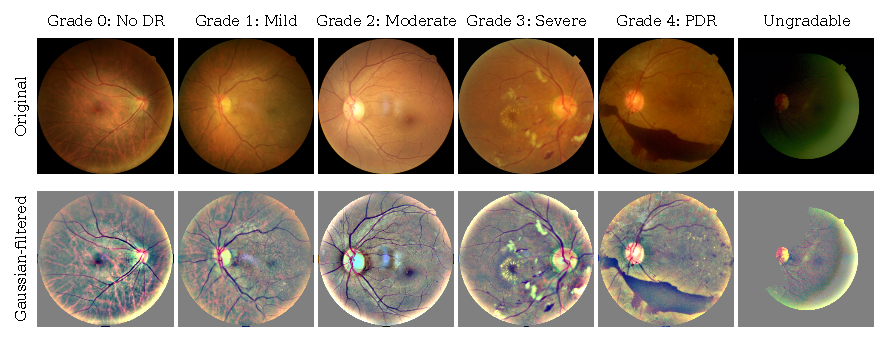
\includegraphics[width=\textwidth]{fig_ddr_samples.pdf}
\caption{Sample DDR fundus images for each grade (top row: cropped original; bottom row: after Gaussian-filter preprocessing). Samples are drawn at random from the training split with a fixed seed, subject to the field of view filling the frame; the last column shows an ungradable image. The preprocessing equalises illumination and exposes vessels and lesions, but amplifies border artefacts.}
\label{fig:ddr-samples}
\end{figure}

\begin{figure}[!htbp]
\centering
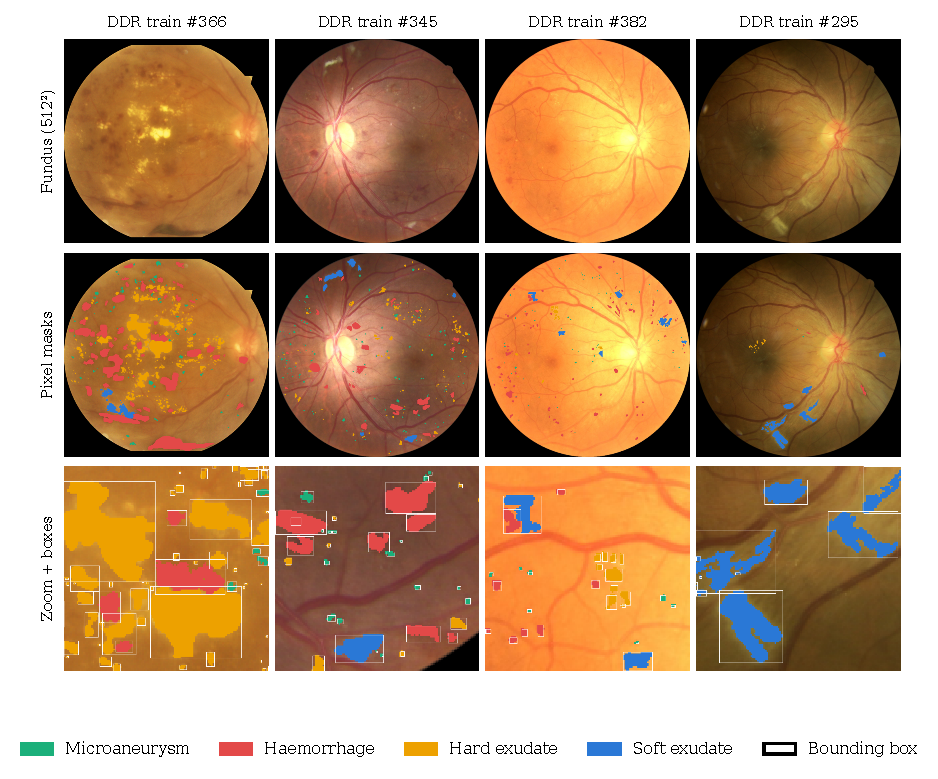
\includegraphics[width=\textwidth]{fig_ddr_lesions.pdf}
\caption{Lesion annotations in four DDR training images that contain several lesion types. Top: fundus image at $512\times512$. Middle: ground-truth pixel masks (MA green, HE red, EX yellow, SE blue). Bottom: densest $128\times128$ window magnified three times with the Pascal-VOC bounding boxes (white). Note the very different sizes and densities of lesions between images.}
\label{fig:ddr-lesions}
\end{figure}

\begin{figure}[!htbp]
\centering
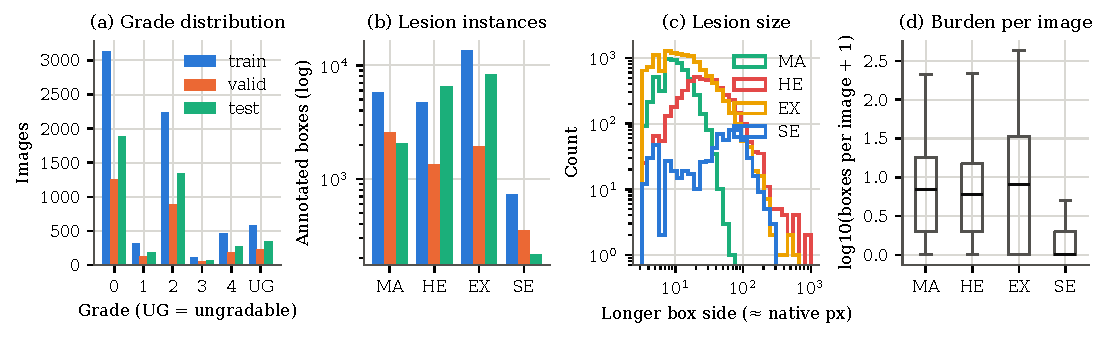
\includegraphics[width=\textwidth]{fig_dataset_stats.pdf}
\caption{Dataset statistics. (a) Grade distribution per split. (b) Number of annotated lesion boxes per class and split (log scale). (c) Distribution of the longer side of lesion boxes in the training set, in approximate native pixels. (d) Lesion burden per image (boxes per image, $\log_{10}$ scale, outliers omitted).}
\label{fig:ddr-stats}
\end{figure}

\subsection{Gaussian-filtered APTOS-derived Kaggle set (external test)}
\label{sec:aptos}
For an external test of the grading pipeline we use the publicly available ``Diabetic Retinopathy 224$\times$224 Gaussian filtered'' Kaggle dataset \citep{rath2020gaussian}, which contains the labelled training portion of the APTOS 2019 Blindness Detection challenge \citep{aptos2019} after resizing to $224\times224$ and Gaussian-filter normalisation in the style of the Kaggle 2015 winning solution \citep{graham2015kaggle}. It contains \num{3664} PNG images in five folders (No\_DR 1805, Mild 370, Moderate 999, Severe 193, Proliferative\_DR 295; CC0 licence). This set differs from DDR in several ways that make it a demanding test of robustness: it originates from a different population and camera set (Aravind Eye Hospital, India), has a different grade distribution (49\% grade~0, 27\% grade~2), has no lesion annotation and, most importantly, has a resolution of only $224\times224$, which removes microaneurysms and most small haemorrhages (Fig.~\ref{fig:aptos}). We therefore \emph{only} use it for zero-shot grading evaluation of models trained on DDR, and not for segmentation or detection. Because the images are already filtered, we apply the same filter to DDR inputs wherever a model is to be transferred (Section~\ref{sec:prep}).

\begin{figure}[!htbp]
\centering
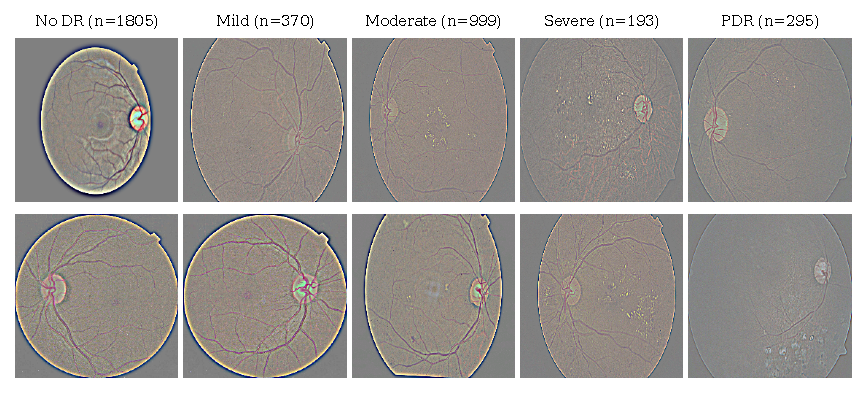
\includegraphics[width=.85\textwidth]{fig_aptos_samples.pdf}
\caption{Random samples (two per grade) from the Gaussian-filtered $224\times224$ APTOS-derived Kaggle set. The Gaussian filter equalises illumination but also removes most colour information; note that some photographs are non-circular owing to the original acquisition.}
\label{fig:aptos}
\end{figure}

\subsection{Preprocessing}
\label{sec:prep}
All photographs are processed as follows. (i) \emph{Border cropping}: the bounding box of pixels whose maximum channel exceeds 12 is cropped and the result is zero-padded to a square, which removes the black margins that occupy a variable portion of DDR frames. (ii) \emph{Resizing}: area interpolation to $512\times512$ for the segmentation network and to $256\times256$ for the image embedding. Binary lesion masks are resized with area interpolation of the floating-point mask followed by a threshold of 0.15, which preserves sub-pixel microaneurysms that nearest-neighbour or threshold-at-0.5 resizing would erase; ground-truth boxes undergo exactly the same geometric transform. (iii) \emph{Gaussian filtering} (optional, denoted ``GF''): $I' = 4I - 4\,(G_{\sigma}\!*\!I) + 128$ with $\sigma = 0.045\,s$ (where $s$ is the image side, matching the common $\sigma\approx10$ at $224$ px), followed by a gray fill outside the field of view. This is the same transform used to produce the Kaggle set, and we study its effect in an ablation (Section~\ref{sec:res-seg}).

\subsection{Data splits, leakage and ethics}
We use the official DDR train/validation/test partition for every task. Model selection (early stopping, thresholds, temperature, conformal calibration) uses validation data only. A subtle point is that the lesion subset is \emph{not} aligned with the grading partition: of the 383 lesion-training images, 275, 100 and 8 belong to the grading training, validation and test partitions, respectively; of the 149 lesion-validation images, 31 are in the grading validation and 118 in the grading test partition; and of the 225 lesion-test images, 152, 12 and 59 are in the grading training, validation and test partitions (Appendix~\ref{app:leak}). Because the segmentation network is fitted on lesion-training images and tuned on lesion-validation images, any grading-test image that belongs to either set would give the lesion branch indirect access to test data. We therefore define a \emph{leak-controlled grading test set} by removing these 126 images (all of which are gradable, grades~1--4), leaving 3633 gradable test images, and report \emph{all} grading test results on this set; results on the full official test partition are given as a sensitivity analysis in Appendix~\ref{app:leak}. Lesion-test images are never used for fitting or selection of the segmentation network, so segmentation and detection results are unaffected. Both datasets are public and de-identified; no new patient data were collected, so institutional review was not required.

\section{Method}
\label{sec:method}

\subsection{Problem formulation and notation}
Let $x\in\R^{H\times W\times 3}$ be a fundus photograph. We consider three coupled tasks on the same input. \emph{Grading} asks for an ordinal grade $y\in\{0,1,2,3,4\}$ (Section~\ref{sec:ddr}). \emph{Segmentation} asks for four binary masks $M_c\in\{0,1\}^{H\times W}$ for lesion classes $c\in\mathcal C=\{\ma,\he,\ex,\se\}$. \emph{Detection} asks for a set of scored boxes $\{(b_j,c_j,s_j)\}$. A segmentation network $f_\phi$ maps the image to lesion probability maps $P=f_\phi(x)\in[0,1]^{4\times H\times W}$; a grading model $g_\psi$ maps the image and the lesion evidence derived from $P$ to cumulative grade probabilities. Table~\ref{tab:notation} lists the main symbols.

\begin{table}[!htbp]
\centering
\caption{Main notation.}
\label{tab:notation}
\small
\begin{tabular}{@{}lp{0.64\textwidth}@{}}
\toprule
Symbol & Meaning \\
\midrule
$x$, $y$ & fundus image, ICDR grade $\in\{0,\dots,4\}$ \\
$\mathcal C=\{\ma,\he,\ex,\se\}$ & lesion classes \\
$P=f_\phi(x)\in[0,1]^{4\times H\times W}$ & lesion probability maps from the segmentation network \\
$\tilde P\in[0,1]^{4\times h\times w}$ & $4\times$ max-pooled maps ($h=w=128$) \\
$\mathcal Z=\{z_1,\dots,z_6\}$, $\Omega_z$ & retinal zones (4 quadrants, central disc, whole field) and their pixel sets \\
$n_{c,z}^{(\tau)},\ \pi_{c,z},\ \mu_{c,z}$ & soft counts at threshold $\tau$, number of peaks, maximum probability \\
$e_{c,z}\in\R^5$, $Z\in\R^{4\times6\times5}$ & evidence vector of $(c,z)$ and the full evidence tensor \\
$\varphi(x)\in\R^{D}$ & frozen image embedding ($D=1152$) \\
$s_k$, $\hat F_k=\sigma(s_k)$ & cumulative logit and probability for the event $y\ge k$, $k=1,\dots,4$ \\
$R_k(Z;\theta)\in[0,1]$ & soft-logic rule score: necessary condition for $y\ge k$ \\
$\sigma_y$, $\lambda$ & soft-label width, rule-loss weight \\
$\mathcal C_\alpha(x)$ & conformal prediction set at miscoverage level $\alpha$ \\
\bottomrule
\end{tabular}
\end{table}

\subsection{Overview}
Fig.~\ref{fig:arch} shows the overall pipeline. The segmentation network is trained on the pixel-annotated DDR subset and applied to every image. Its probability maps are summarised by the lesion-evidence bottleneck into a tensor $Z$ of soft, zone-wise lesion statistics (Section~\ref{sec:evidence}). The grading head combines a frozen embedding of the same image with the evidence tokens through a transformer (Section~\ref{sec:head}) and outputs cumulative ordinal probabilities (Section~\ref{sec:ordinal}). A rule module computes ICDR-style necessary-condition scores $R_k(Z)$ and penalises predictions that exceed them (Section~\ref{sec:rule}). Probabilities are temperature-scaled and converted into conformal prediction sets (Section~\ref{sec:conformal}). Detection boxes are obtained from the same probability maps $P$ (Section~\ref{sec:det}).

\begin{figure}[!htbp]
\centering
\resizebox{\textwidth}{!}{%
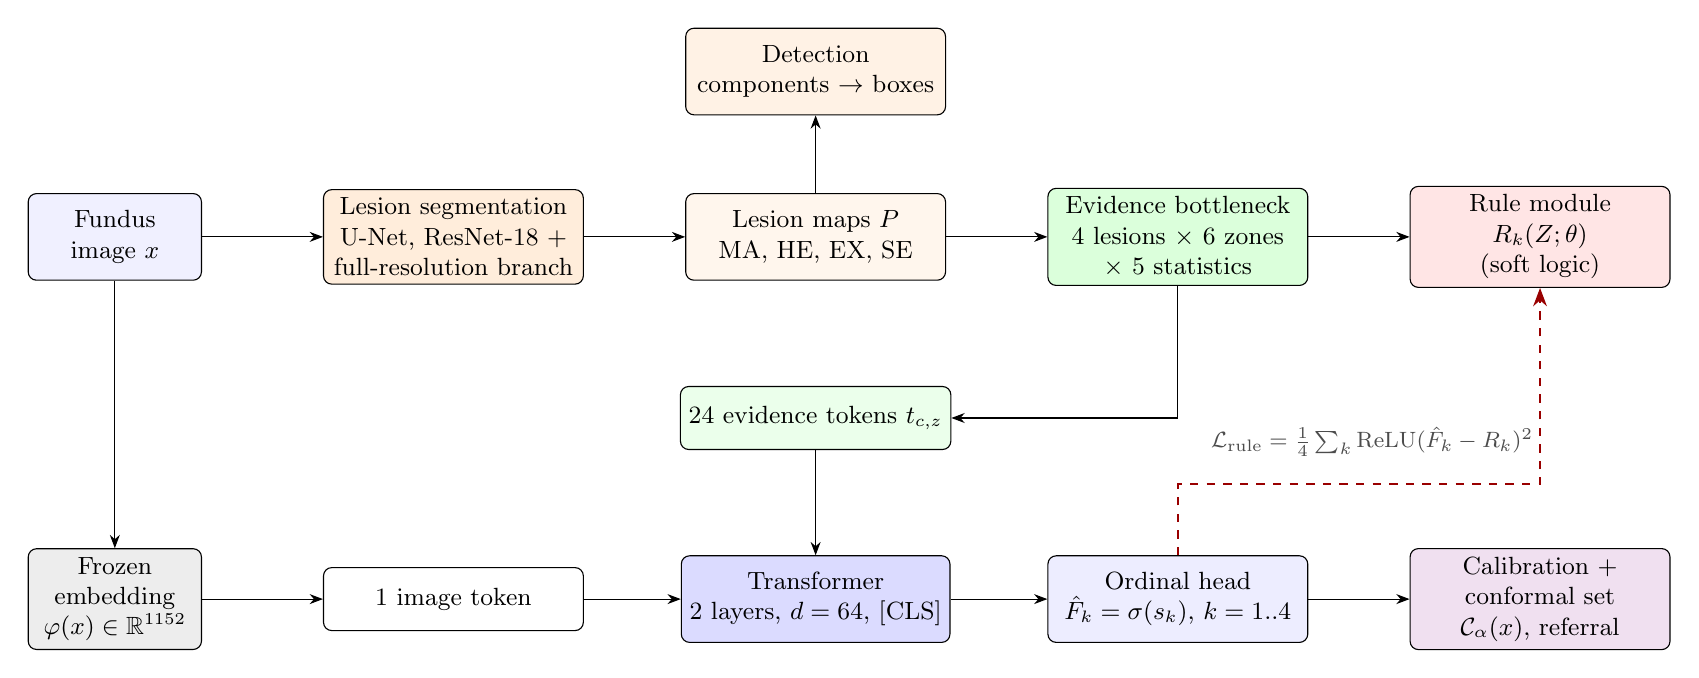
\begin{tikzpicture}[
  >=Stealth, font=\small,
  blk/.style={draw, rounded corners=3pt, minimum height=11mm, minimum width=33mm, align=center, inner sep=3pt, fill=#1},
  lab/.style={font=\footnotesize\itshape, text=black!70}]
% row A: segmentation branch
\node[blk=blue!6, minimum width=22mm] (img) at (0,0) {Fundus\\image $x$};
\node[blk=orange!14] (seg) at (4.3,0) {Lesion segmentation\\U-Net, ResNet-18 +\\full-resolution branch};
\node[blk=orange!7] (maps) at (8.9,0) {Lesion maps $P$\\MA, HE, EX, SE};
\node[blk=green!14] (evi) at (13.5,0) {Evidence bottleneck\\4 lesions $\times$ 6 zones\\$\times$ 5 statistics};
\node[blk=red!10] (rule) at (18.1,0) {Rule module\\$R_k(Z;\theta)$\\(soft logic)};
\node[blk=orange!10] (det) at (8.9,2.1) {Detection\\components $\to$ boxes};
% row B: grading branch
\node[blk=gray!14, minimum width=22mm] (emb) at (0,-4.6) {Frozen\\embedding\\$\varphi(x)\in\R^{1152}$};
\node[blk=white, minimum height=8mm] (itok) at (4.3,-4.6) {1 image token};
\node[blk=green!8, minimum height=8mm] (tok) at (8.9,-2.3) {24 evidence tokens $t_{c,z}$};
\node[blk=blue!14] (tr) at (8.9,-4.6) {Transformer\\2 layers, $d=64$, [CLS]};
\node[blk=blue!7] (ord) at (13.5,-4.6) {Ordinal head\\$\hat F_k=\sigma(s_k)$, $k=1..4$};
\node[blk=violet!12] (conf) at (18.1,-4.6) {Calibration +\\conformal set\\$\mathcal C_\alpha(x)$, referral};
\draw[->] (img) -- (seg); \draw[->] (seg) -- (maps); \draw[->] (maps) -- (evi); \draw[->] (evi) -- (rule);
\draw[->] (maps) -- (det);
\draw[->] (img) -- (emb); \draw[->] (emb) -- (itok); \draw[->] (itok) -- (tr);
\draw[->] (evi.south) |- (tok.east); \draw[->] (tok) -- (tr);
\draw[->] (tr) -- (ord); \draw[->] (ord) -- (conf);
\draw[->, dashed, red!60!black, thick] (ord.north) -- ++(0,0.9) -| (rule.south);
\node[lab, anchor=west] at (13.8,-2.6) {$\mathcal L_{\mathrm{rule}}=\frac14\sum_k\mathrm{ReLU}(\hat F_k-R_k)^2$};
\end{tikzpicture}}
\caption{Overview of \mname. A segmentation network produces lesion maps; a differentiable bottleneck turns them into zone-wise evidence tokens, which a transformer combines with a frozen image embedding to predict cumulative ordinal probabilities. A soft-logic rule module (dashed) penalises grades that the lesion evidence cannot justify. Probabilities are calibrated and wrapped into conformal sets. The same lesion maps yield detection boxes.}
\label{fig:arch}
\end{figure}

\subsection{Lesion segmentation network}
\label{sec:seg}
\paragraph{Architecture.} The segmenter $f_\phi$ is a U-Net \citep{ronneberger2015} with a ResNet-18 encoder \citep{he2016resnet} initialised from ImageNet weights (as distributed in \texttt{timm} \citep{wightman2019timm}). The encoder produces features at strides 2, 4, 8, 16 and 32; the decoder upsamples bilinearly and fuses encoder features by concatenation followed by two $3\times3$ convolution--BN--ReLU blocks (widths 128, 96, 64, 48). Because micro-aneurysms are only a few pixels wide, stride-2 features are not sufficient, and we add a shallow \emph{full-resolution branch} (two $3\times3$ conv--BN--ReLU blocks with 16 channels applied directly to the input) whose output is concatenated with the upsampled decoder output before a final $3\times3$ block and a $1\times1$ convolution to four logits. The network has 11.8\,M parameters.

\paragraph{Objective.} Let $p_c=\sigma(\ell_c)$ be the predicted probability map and $y_c$ the binary mask of class $c$. We compare three objectives:
\begin{align}
\mathcal L_{\mathrm{bce}} &= \tfrac14\textstyle\sum_{c}\mathrm{BCE}(p_c,y_c),\\
\mathcal L_{\mathrm{bce+dice}} &= \tfrac14\textstyle\sum_{c}\big[\mathrm{BCE}_w(p_c,y_c) + \mathcal L_{\mathrm{Dice}}(p_c,y_c)\big],\\
\mathcal L_{\mathrm{seg}} &= \tfrac14\textstyle\sum_{c}\big[\mathrm{BCE}_w(p_c,y_c) + 2\,\mathrm{FTL}_c\big],
\end{align}
where $\mathrm{BCE}_w$ weights positive pixels by $w=(20,6,6,8)$ for (MA, HE, EX, SE), reflecting that the smaller and rarer the lesion class, the stronger the class imbalance. $\mathcal L_{\mathrm{Dice}}=1-\frac{2\sum p y+1}{\sum p+\sum y+1}$, and the focal Tversky loss \citep{abraham2019ftl,salehi2017tversky} is
\begin{equation}
\mathrm{FTL}_c=\Big(1-\mathrm{TI}_c\Big)^{\gamma},\qquad \mathrm{TI}_c=\frac{\mathrm{TP}_c+1}{\mathrm{TP}_c+\alpha\,\mathrm{FP}_c+\beta\,\mathrm{FN}_c+1},
\label{eq:ftl}
\end{equation}
with $\mathrm{TP}_c=\sum p_c y_c$, $\mathrm{FP}_c=\sum p_c(1-y_c)$, $\mathrm{FN}_c=\sum(1-p_c)y_c$ computed over the mini-batch, $\alpha=0.3$, $\beta=0.7$ and $\gamma=0.75$. Since $\beta>\alpha$, missed lesion pixels cost more than spurious ones, which is the desirable bias for screening where recall of small lesions dominates; $\gamma<1$ gives larger gradients to well-classified classes than the plain Tversky loss, and keeps the loss sensitive when overlap is already moderate. $\mathcal L_{\mathrm{seg}}$ is the default objective used below; $\mathcal L_{\mathrm{bce}}$ and $\mathcal L_{\mathrm{bce+dice}}$ are the ablation baselines. We make no a-priori claim that the focal Tversky objective is superior to Dice: Section~\ref{sec:res-seg} reports the comparison.

\paragraph{Lesion-centred sampling and optimisation.} Positive pixels are less than 1\% of all pixels. Each training crop ($256\times256$) is, with probability 0.7, positioned around a pixel of a randomly chosen lesion class in an image containing that class (the offset of the lesion inside the crop is random), and with probability 0.3 sampled uniformly. We use random flips, $90^\circ$ rotations and brightness/contrast jitter. Optimisation uses AdamW \citep{loshchilov2019adamw} with weight decay $10^{-4}$, one-cycle learning-rate schedule (peak $10^{-3}$, 15\% warm-up), batches of 8 crops, 48 iterations per epoch, 30 epochs and bfloat16 autocast on CPU (Alg.~\ref{alg:seg}). The checkpoint with the highest mean AUPR on the lesion-validation split (evaluated every five epochs at the full $512\times512$ resolution) is retained.

\begin{algorithm}[!htbp]
\caption{Lesion-centred training of the segmentation network.}
\label{alg:seg}
\begin{algorithmic}[1]
\Require lesion-train images $\{(x_i,Y_i)\}$, epochs $E$, iterations $I$, crop size $q$, probability $\rho=0.7$
\For{$e=1,\dots,E$}
  \For{$t=1,\dots,I$}
    \For{$b=1,\dots,8$}
      \State draw $u\sim\mathcal U(0,1)$
      \If{$u<\rho$} \State draw class $c$, image $i$ with $Y_{i,c}\neq0$, lesion pixel $r$; place crop containing $r$ at a random offset
      \Else \State draw image $i$ and crop position uniformly \EndIf
      \State augment (flip, rot$90^\circ$, brightness/contrast) crop and mask
    \EndFor
    \State $\ell\gets f_\phi(\text{batch})$ (bf16); $\mathcal L\gets \mathcal L_{\mathrm{seg}}(\ell,\text{masks})$ with Eq.~\eqref{eq:ftl}
    \State update $\phi$ with AdamW and one-cycle schedule
  \EndFor
  \If{$e\bmod5=0$} \State evaluate mean AUPR on lesion-valid at $512^2$; keep best $\phi$ \EndIf
\EndFor
\end{algorithmic}
\end{algorithm}

\subsection{Detection from segmentation maps}
\label{sec:det}
For a class $c$ and image, the probability map $P_c$ is thresholded at a class-specific seed threshold $\vartheta_c$. Each 8-connected component $K$ of $\{u:P_c(u)\ge\vartheta_c\}$ becomes a box $b_K$ (its tight bounding rectangle) with score $s_K=\frac{1}{|K|}\sum_{u\in K}P_c(u)$. Because the segmentation objective is trained with positive-class weights, probabilities are not calibrated and the Dice-optimal threshold is high (typically $>0.8$); using it as seed would cap the attainable recall. We therefore choose $\vartheta_c$ from the grid $\Theta=\{0.05,0.1,0.2,0.3,0.5,0.7\}$ by maximising AP at IoU 0.3 on the lesion-\emph{validation} split. Lower seeds have higher recall but more false positives; the scores order the boxes for precision--recall and FROC analysis (Alg.~\ref{alg:det}). No extra network is trained: segmentation and detection share the same weights, and we evaluate the proposals directly against the DDR ground-truth boxes.

\begin{algorithm}[!htbp]
\caption{Segmentation-guided lesion proposals and evaluation.}
\label{alg:det}
\begin{algorithmic}[1]
\Require probability maps $P\in[0,1]^{4\times H\times W}$, seed grid $\Theta$, validation split with ground-truth boxes
\For{each class $c\in\mathcal C$}
  \State $\vartheta_c\gets\arg\max_{\vartheta\in\Theta}\mathrm{AP}_{0.3}^{\text{val}}(\vartheta)$ (computed once on validation images); $B_c\gets\emptyset$
  \State find 8-connected components $\{K\}$ of $\{u:P_c(u)\ge\vartheta_c\}$
  \For{each component $K$}
    \State $b_K\gets$ bounding box of $K$; $s_K\gets\operatorname{mean}_{u\in K}P_c(u)$; add $(b_K,s_K)$ to $B_c$
  \EndFor
\EndFor
\State \textbf{evaluate}: sort $B_c$ by score; greedy one-to-one matching to unique ground-truth boxes with $\mathrm{IoU}\ge\kappa$ (AP$_\kappa$, $\kappa\in\{0.3,0.5\}$); lesion-level FROC: a box is a hit if its centre lies inside a ground-truth box
\end{algorithmic}
\end{algorithm}

\subsection{Lesion-evidence bottleneck}
\label{sec:evidence}
The grading head does not see $P$ directly; it sees a compact, interpretable summary computed as follows.

\paragraph{Zones.} Let $h=w=128$ and let $\tilde P=\mathrm{maxpool}_{4}(P)\in[0,1]^{4\times h\times w}$. Max-pooling (rather than average pooling) keeps the peak of a one-pixel microaneurysm. We define six zones with binary masks $\Omega_z$ on the $h\times w$ grid, restricted to the circular field of view of radius $0.5h-2$: four quadrants (split by the horizontal and vertical lines through the image centre), a central disc of radius $0.35\cdot(h/2)$ approximating the macular region, and the whole field. Because the cropped photographs are approximately centred on the optic disc--macula axis, quadrants are a pragmatic stand-in for the ETDRS/ICDR quadrant definition; we do not claim anatomical registration.

\paragraph{Soft counts.} Counting connected components is not differentiable and is unstable under thresholding. Instead, for threshold levels $\tau\in\{0.25,0.5,0.75\}$ we compute
\begin{equation}
n_{c,z}^{(\tau)}=\sum_{u\in\Omega_z}\sigma\!\Big(\frac{\tilde P_c(u)-\tau}{T}\Big),\qquad T=0.05,
\label{eq:softcount}
\end{equation}
which counts the number of pooled cells in zone $z$ that contain lesion class $c$ with confidence about $\tau$. Two further statistics are the number of local peaks $\pi_{c,z}=\sum_{u\in\Omega_z}\mathbb 1[\tilde P_c(u)=\max_{u'\in\mathcal N_3(u)}\tilde P_c(u')\wedge \tilde P_c(u)>0.5]$ (a proxy for the lesion count) and the maximum probability $\mu_{c,z}=\max_{u\in\Omega_z}\tilde P_c(u)$. The evidence vector is
\begin{equation}
e_{c,z}=\log\!\big(1+\big[n_{c,z}^{(0.25)},\,n_{c,z}^{(0.5)},\,n_{c,z}^{(0.75)},\,\pi_{c,z},\,10\,\mu_{c,z}\big]\big)\in\R^5,
\label{eq:evidence}
\end{equation}
and the tensor $Z=(e_{c,z})\in\R^{4\times6\times5}$ (120 numbers) is the \emph{only} way in which lesion information enters the grade (Alg.~\ref{alg:evid}). The logarithm compresses the dynamic range between a handful of microaneurysms and several hundred exudate cells. Since Eq.~\eqref{eq:softcount} is smooth in $\tilde P$, the bottleneck is differentiable in principle, which would allow end-to-end fine-tuning of $f_\phi$ from grade supervision; in the present study, $f_\phi$ is frozen at this stage for compute reasons (Section~\ref{sec:setup}).

\begin{algorithm}[!htbp]
\caption{Zone-wise soft lesion evidence.}
\label{alg:evid}
\begin{algorithmic}[1]
\Require lesion probability maps $P\in[0,1]^{4\times H\times W}$, zone masks $\{\Omega_z\}_{z=1}^{6}$ on the $128^2$ grid
\State $\tilde P\gets\operatorname{maxpool}_4(P)$
\For{$c\in\mathcal C$, $z=1..6$}
  \For{$\tau\in\{0.25,0.5,0.75\}$} \State $n^{(\tau)}_{c,z}\gets\sum_{u\in\Omega_z}\sigma\big((\tilde P_c(u)-\tau)/T\big)$ \EndFor
  \State $\pi_{c,z}\gets\sum_{u\in\Omega_z}\mathbb 1[\tilde P_c(u)\text{ is a }3{\times}3\text{ local maximum},\ \tilde P_c(u)>0.5]$
  \State $\mu_{c,z}\gets\max_{u\in\Omega_z}\tilde P_c(u)$
  \State $e_{c,z}\gets\log(1+[n^{(.25)},n^{(.5)},n^{(.75)},\pi,10\mu])$
\EndFor
\State \Return $Z=(e_{c,z})$
\end{algorithmic}
\end{algorithm}

\subsection{Evidence-token grade head}
\label{sec:head}
Each $(c,z)$ pair becomes a token $t_{c,z}=W_e\,e_{c,z}+a_c+b_z\in\R^d$ with $d=64$, where $a_c$ and $b_z$ are learned class and zone embeddings. The frozen image embedding $\varphi(x)\in\R^{1152}$ (concatenated global averages of stages 3 and 4 of a ConvNeXt-T \citep{liu2022convnext} applied to the $256\times256$ filtered image, standardised with training-set statistics) becomes one image token $t_0=W_i\,\mathrm{Dropout}(\varphi(x))$. A learned [CLS] token and the $1+24$ tokens enter a two-layer pre-LN transformer encoder (four heads, feed-forward width 128, dropout 0.1). The output of the [CLS] token passes through LayerNorm and a linear layer to produce four cumulative logits $s_1,\dots,s_4$. Attention weights from the [CLS] token to the evidence tokens provide a direct, inspectable account of which lesion class and zone drove a prediction. The head has 0.14\,M parameters, so that the whole grading stage can be trained in seconds on a CPU.

\subsection{Ordinal cumulative-link objective with soft targets}
\label{sec:ordinal}
Following the multiple-output formulation of ordinal regression \citep{niu2016ordinal,cao2020coral}, we model $\hat F_k=P(y\ge k\mid x)=\sigma(s_k)$ for $k=1,\dots,4$. To model adjacent-grade disagreement we replace the one-hot target by a discretised Gaussian over grades,
\begin{equation}
q_j(y)=\frac{\exp\!\big(-(j-y)^2/2\sigma_y^2\big)}{\sum_{j'=0}^{4}\exp\!\big(-(j'-y)^2/2\sigma_y^2\big)},\quad
F_k^\star=\sum_{j\ge k}q_j(y),
\label{eq:softlabel}
\end{equation}
and minimise the binary cross-entropy between $F_k^\star$ and $\hat F_k$:
\begin{equation}
\mathcal L_{\mathrm{ord}}=-\frac14\sum_{k=1}^{4}\Big[F^\star_k\log\hat F_k+(1-F^\star_k)\log(1-\hat F_k)\Big].
\label{eq:ord}
\end{equation}
With $\sigma_y=0$ this reduces to the standard cumulative-link loss. At inference, $\hat y=\sum_k\mathbb 1[\hat F_k>0.5]$, and the class probabilities are obtained from the monotonised cumulative probabilities $\bar F_k=\min_{k'\le k}\hat F_{k'}$ as $p_j=\bar F_j-\bar F_{j+1}$ (with $\bar F_0=1$, $\bar F_5=0$), floored at $10^{-6}$ and renormalised. In our experiments, $\sigma_y=0.5$, which places about 0.79 of the target mass on the labelled grade and 0.10 on each neighbour.

\subsection{Clinical-rule consistency}
\label{sec:rule}
The ICDR scale describes grades through necessary conditions on the lesions that must be visible. We encode four such conditions as soft logic \citep{diligenti2017sbr,hu2016logic}, using the product t-norm for conjunction ($a\wedge b=ab$) and its dual for disjunction ($a\vee b=1-(1-a)(1-b)$). Let $u_{c,z}=e_{c,z,2}=\log(1+n_{c,z}^{(0.5)})$ and $a(v;\theta)=\sigma((v-\theta)/s)$ with $s=0.35$. With learnable thresholds $\theta=(\theta_1,\dots,\theta_{10})$ and $z=\mathrm{all}$ the whole-field zone, the rule scores are
\begin{align}
R_1&=\textstyle\bigvee_{c\in\mathcal C}\,a(u_{c,\mathrm{all}};\theta_{c}),\label{eq:r1}\\
R_2&=a(u_{\ma,\mathrm{all}};\theta_5)\vee a(u_{\he,\mathrm{all}};\theta_2)\vee a(u_{\ex,\mathrm{all}};\theta_3)\vee a(u_{\se,\mathrm{all}};\theta_4),\label{eq:r2}\\
R_3&=\Big(\textstyle\bigwedge_{q=1}^{4}a(u_{\he,q};\theta_{5+q})\Big)\vee a(u_{\se,\mathrm{all}};\theta_{10}),\label{eq:r3}\\
R_4&=R_2,\label{eq:r4}
\end{align}
where $\theta_c$ in Eq.~\eqref{eq:r1} denotes the thresholds $\theta_1,\dots,\theta_4$ for $c=\ma,\he,\ex,\se$. The four rules read as follows. $R_1$: some lesion is visible (needed for mild DR or worse). $R_2$: lesions beyond a few microaneurysms are visible (needed for moderate or worse). $R_3$: haemorrhages in all four quadrants, \emph{or} extensive soft exudates (a soft proxy for the ``4'' of the 4--2--1 rule; needed for severe or worse). $R_4$: proliferative DR is never lesion-free.
Venous beading, IRMA and neovascularisation are not annotated in DDR, so $R_3$ is only a partial surrogate and $R_4$ imposes just a weak necessary condition. We stress that these rules are \emph{necessary conditions} (``$y\ge k\Rightarrow R_k$''), not sufficient ones: a grade may be lower than the lesions allow, but never higher.

\paragraph{Calibrating thresholds on labels.} Because the predicted lesion statistics are noisy, hand-set thresholds would be arbitrary. We therefore fit $\theta$ once on the training labels by minimising
\begin{equation}
\mathcal L_{\mathrm{fit}}(\theta)=\sum_{k=1}^{4}\Big[\E_{i:\,y_i\ge k}\big(1-R_k(Z_i;\theta)\big)+\tfrac12\,\E_{i:\,y_i<k}R_k(Z_i;\theta)\Big],
\label{eq:rulefit}
\end{equation}
that is, the rule should hold for images whose grade is at least $k$ (first term), and should not hold trivially for lesion-poor images (second term, which prevents $R_k\equiv1$). The parameters are then frozen. The rules are thus \emph{clinically inspired, data-calibrated templates}, not a re-implementation of the grading guideline.

\paragraph{Rule-consistency loss and violation rate.} The grading head is trained with
\begin{equation}
\mathcal L=\mathcal L_{\mathrm{ord}}+\lambda\,\mathcal L_{\mathrm{rule}},\qquad
\mathcal L_{\mathrm{rule}}=\frac14\sum_{k=1}^4\mathrm{ReLU}\big(\hat F_k-R_k(Z;\theta)\big)^2,\quad\lambda=1,
\label{eq:total}
\end{equation}
so that the predicted probability of grade $\ge k$ is pushed below the rule score. As an evaluation measure independent of the training loss, we define the \emph{rule-violation rate} of a model $\hat y(\cdot)$ on a test set as the fraction of images for which $\hat y\ge k$ and $R_k<0.5$ for at least one $k\le\hat y$ (Alg.~\ref{alg:rule}); the same frozen rules are applied to \emph{every} model, including baselines that never saw them.

\begin{algorithm}[!htbp]
\caption{Rule calibration, rule-consistent training and violation rate.}
\label{alg:rule}
\begin{algorithmic}[1]
\Require training evidence $\{Z_i\}$, labels $\{y_i\}$, embeddings $\{\varphi_i\}$, $\sigma_y$, $\lambda$
\State \textbf{Calibrate rules:} initialise $\theta$; minimise $\mathcal L_{\mathrm{fit}}(\theta)$ (Eq.~\ref{eq:rulefit}) with Adam; freeze $\theta$
\For{epoch $=1,\dots,60$}
  \For{mini-batch $B$}
    \State $s\gets g_\psi(\varphi,Z)$; $\hat F\gets\sigma(s)$
    \State $\mathcal L\gets\mathcal L_{\mathrm{ord}}(\hat F,F^\star(y;\sigma_y))+\lambda\cdot\frac14\sum_k\mathrm{ReLU}(\hat F_k-R_k(Z;\theta))^2$
    \State update $\psi$ (AdamW, cosine schedule)
  \EndFor
  \State every 3 epochs: compute quadratic-weighted kappa on validation half A; keep best $\psi$
\EndFor
\State \textbf{Violation rate} on test set: $\frac1N\sum_i\mathbb 1[\exists k\le\hat y_i:\ R_k(Z_i;\theta)<0.5]$
\end{algorithmic}
\end{algorithm}

\subsection{Calibration and split-conformal referral}
\label{sec:conformal}
\paragraph{Temperature scaling.} On validation half A we fit a single temperature $T^\star\in[0.5,3]$ that minimises the negative log-likelihood of the class probabilities obtained from the logits $s_k/T$ \citep{guo2017calibration}; this changes confidences but not predicted grades. Expected calibration error (ECE) is computed with 15 equal-width confidence bins.

\paragraph{Split-conformal sets.} Let $\hat p(x)\in\Delta^4$ denote the calibrated class probabilities. On validation half B (calibration set of size $n$, disjoint from model selection and temperature fitting), we define the nonconformity score $\varsigma_i=1-\hat p_{y_i}(x_i)$ and the threshold
\begin{equation}
\hat q_\alpha=\varsigma_{(\lceil(n+1)(1-\alpha)\rceil)},\qquad
\mathcal C_\alpha(x)=\{j:\ 1-\hat p_j(x)\le\hat q_\alpha\},
\label{eq:conformal}
\end{equation}
where $\varsigma_{(m)}$ is the $m$-th smallest score. If calibration and test data are exchangeable, $\Pr[y\in\mathcal C_\alpha(x)]\ge1-\alpha$ marginally \citep{vovk2005,angelopoulos2023}. Sets of size one are confident decisions; larger sets signal ambiguity. We define a \emph{referral rule}: refer the patient if $\mathcal C_\alpha(x)$ contains any grade $\ge2$ (referable DR); because the guarantee concerns the true grade, the probability that a truly referable patient is \emph{not} referred is at most $\alpha$ \emph{marginally over the population}, but it need not hold within each class. We therefore also report the empirical class-conditional referral sensitivity (Alg.~\ref{alg:conf}).

\begin{algorithm}[!htbp]
\caption{Calibration and split-conformal referral.}
\label{alg:conf}
\begin{algorithmic}[1]
\Require trained head, validation halves A and B, test image $x$, level $\alpha$
\State $T^\star\gets\arg\min_{T}\mathrm{NLL}(\text{half A};T)$
\State for $i\in$ half B: $\varsigma_i\gets 1-\hat p_{y_i}(x_i;T^\star)$
\State $\hat q_\alpha\gets$ the $\lceil(n+1)(1-\alpha)\rceil$-th smallest $\varsigma_i$
\State $\mathcal C_\alpha(x)\gets\{j:\ 1-\hat p_j(x;T^\star)\le\hat q_\alpha\}$
\State \textbf{refer} iff $\max\mathcal C_\alpha(x)\ge2$
\end{algorithmic}
\end{algorithm}

\subsection{Image-quality gate}
\label{sec:quality}
Under the six-class protocol, ungradable images (grade~5 in DDR) are detected by a separate binary classifier with the same MLP architecture as the baseline, trained on all training images with the target $\mathbb 1[y=5]$. Its decision threshold is chosen on validation data to maximise the macro-F1 of the six-class prediction; an image flagged as ungradable receives class~5, otherwise the ordinal grade is output. The gate is deliberately kept independent of the ordinal head, so that the five-class results are not affected by it.

\subsection{Complexity}
The segmentation network (11.8\,M parameters) is the dominant cost: on four CPU cores with bfloat16 it processes about 8 images per second at $512\times512$ (Section~\ref{sec:setup}). Evidence extraction (Alg.~\ref{alg:evid}) costs $\mathcal O(4\cdot6\cdot h w)$ per image and is negligible. The grading head has 0.14\,M parameters, and each ordinal prediction needs 26 tokens, i.e. $\mathcal O(26^2 d)$ attention operations. Conformal calibration needs a sort of $n$ scores. The method thus adds under 1\% of parameters and well under 1\% of the compute of the segmentation network on top of a backbone embedding.

\section{Experimental setup}
\label{sec:setup}

\subsection{Compute environment and its consequences}
All experiments were run on a single cloud virtual machine with four CPU cores of an Intel Xeon (2.1\,GHz, AVX-512 and AMX bfloat16 instructions), 15\,GB of memory and no GPU. PyTorch \citep{paszke2019pytorch} with bfloat16 autocast and channels-last tensors gave a $3$--$4\times$ speed-up over float32 on this hardware, which made the following design feasible: the segmentation network trains in about 23 minutes (30 epochs) and processes about eight $512\times512$ images per second at inference. Image embeddings come from a \emph{frozen} ImageNet-pretrained backbone, so that the grading stage trains in seconds and can be repeated over many seeds. This design imposes limitations that readers should keep in mind: (i) the segmentation network is trained at $512\times512$ rather than at native resolution (about $1950\times1950$), which shrinks microaneurysms to one to three pixels; (ii) it is trained on the 383 lesion-training images only; (iii) the image backbone is not fine-tuned on DR; (iv) segmentation results come from a single training run per configuration (seed 0), while grading-stage results average five seeds; and (v) heavy detectors (Faster R-CNN, DETR) and large transformer backbones could not be trained within the budget, so detection is evaluated through segmentation-derived proposals against a classical image-processing baseline and across segmentation losses.

\subsection{Implementation details}
\paragraph{Segmentation} Architecture, losses, sampling and optimisation are as described in Section~\ref{sec:seg}. Variants trained: (a) $\mathcal L_{\mathrm{bce}}$, (b) $\mathcal L_{\mathrm{bce+dice}}$, (c) $\mathcal L_{\mathrm{seg}}$ (focal Tversky) on raw colour input, and (d) $\mathcal L_{\mathrm{seg}}$ on Gaussian-filtered input (``GF''; Section~\ref{sec:prep}). All use the same seed, crop sampler and schedule. Thresholds for Dice/IoU are chosen on lesion-validation data per class.

\paragraph{Image embedding} ConvNeXt-T (ImageNet-1k weights \texttt{convnext\_tiny.fb\_in1k} from \texttt{timm}) is applied to $256\times256$ Gaussian-filtered images; global averages of stage 3 (384 channels) and stage 4 (768 channels) are concatenated to a 1152-dimensional vector and standardised using training-set statistics. We chose this backbone and resolution a priori for throughput reasons; no alternative was evaluated on the test set.

\paragraph{Grading heads} All heads are trained with AdamW (weight decay 0.01), cosine schedule over 60 epochs, mini-batches of 128, with learning rate $10^{-3}$ for MLPs and $5\times10^{-4}$ for the token head; the epoch with the highest quadratic-weighted kappa on validation half A (checked every three epochs) is retained. Validation is split into two halves with a fixed random permutation: half~A (1251 images) for model selection and temperature, half~B (1252 images) for conformal calibration. Each configuration is trained with five seeds (0--4); the data split is the same for all.

\subsection{Compared methods}
Table~\ref{tab:methods} lists the grading models. B1--B4 share the same embedding and (where applicable) the same lesion evidence as the proposed models, so that every difference is attributable to \emph{how} lesion information is used.

\begin{table}[!htbp]
\centering
\caption{Grading models compared. All use the same frozen ConvNeXt-T embedding $\varphi(x)$; ``evidence'' means the tensor $Z$ derived from the segmentation maps of the same segmentation network.}
\label{tab:methods}
\small
\begin{tabularx}{\textwidth}{@{}l>{\raggedright\arraybackslash}Xcccc@{}}
\toprule
Model & Description & Evidence & Ordinal & Soft & Rule \\
\midrule
B1 & MLP on $\varphi(x)$, 5-way cross-entropy & -- & -- & -- & -- \\
B2 & MLP on $\varphi(x)$, cumulative-link loss (Eq.~\ref{eq:ord}, $\sigma_y=0$) & -- & \checkmark & -- & -- \\
B3 & MLP on the flattened evidence $Z$ only & \checkmark & \checkmark & -- & -- \\
B4 & MLP on concatenation $[\varphi(x),Z]$ (naive fusion) & \checkmark & \checkmark & -- & -- \\
T0 & Evidence-token transformer, $\sigma_y=0$, $\lambda=0$ & \checkmark & \checkmark & -- & -- \\
T1 & T0 with soft targets ($\sigma_y=0.5$) & \checkmark & \checkmark & \checkmark & -- \\
T2 & T0 with rule loss ($\lambda=1$) & \checkmark & \checkmark & -- & \checkmark \\
\textbf{\mname} & transformer, $\sigma_y=0.5$, $\lambda=1$ & \checkmark & \checkmark & \checkmark & \checkmark \\
A1 & \mname\ without evidence tokens in the head (image token only; rule loss still reads $Z$) & (rule only) & \checkmark & \checkmark & \checkmark \\
\bottomrule
\end{tabularx}
\end{table}

For segmentation, the four U-Net variants of Section~\ref{sec:seg} are compared. For detection we compare segmentation-derived proposals from each variant and a classical baseline: top-hat filtering of the green channel followed by threshold and connected components (dark top-hat for MA and HE, bright top-hat for EX and SE), with the threshold tuned per class on lesion-validation data. We do not compare against published numbers of other systems because their splits, resolutions and training budgets differ.

\subsection{Evaluation metrics}
\paragraph{Grading} The primary metric is the quadratic-weighted Cohen's kappa (QWK) \citep{cohen1968kappa}, the standard agreement measure for ordinal DR grades. We also report accuracy, macro-averaged F1, the area under the ROC curve (AUC) for referable DR ($y\ge2$) computed from $P(y\ge2)$, expected calibration error (ECE, 15 bins), and the rule-violation rate (Section~\ref{sec:rule}). Conformal prediction is evaluated at $\alpha\in\{0.05,0.1,0.2\}$ by empirical coverage, mean set size, singleton fraction and referral sensitivity/specificity. All grading metrics are computed on the leak-controlled test set (Section~\ref{sec:data}) unless stated.

\paragraph{Segmentation} The area under the precision--recall curve (AUPR) of the pixel probabilities, computed exactly after quantising probabilities to 512 levels, is the primary metric because it is threshold-free and appropriate for extreme class imbalance \citep{saito2015pr}. We additionally report Dice \citep{dice1945} and intersection-over-union (IoU) at the per-class validation-optimal threshold, accumulated over all test pixels.

\paragraph{Detection} Average precision at IoU 0.5 and 0.3 (all-point interpolation \citep{padilla2021detmetrics}) and lesion-level FROC sensitivity at 1, 2, 4, 8 and 16 false positives per image, where a prediction is a hit if its centre lies in a ground-truth box. The relaxed IoU of 0.3 is reported because, for a box a few pixels wide, one pixel of displacement lowers IoU dramatically.

\subsection{Statistical analysis}
Grading results are reported as mean $\pm$ standard deviation over five seeds. For the main comparisons we additionally report 95\% confidence intervals obtained by a non-parametric bootstrap of the test images \citep{efron1993bootstrap} (2000 resamples) applied to the seed-averaged class probabilities, and paired bootstrap differences in QWK between models, which respect the pairing of test images. Differences are deemed significant when the 95\% interval of the paired difference excludes zero; no multiplicity correction is applied to the exploratory ablation table, and we say so where relevant. Segmentation metrics are reported from a single run per configuration; we therefore do not make significance claims among segmentation variants and we compare them descriptively.

\subsection{Reproducibility}
All scripts (data extraction, training, evaluation, figure and table generation) and intermediate artefacts (cached lesion maps, embeddings, per-seed probabilities) are released with the paper. Every number in the tables is generated by scripts from stored result files; there is no manual transcription. Random seeds are fixed. The code reads the DDR archive directly from its split zip volumes, so no re-packaging is needed.

\section{Results}
\label{sec:results}
We report segmentation and detection first (Sections~\ref{sec:res-seg} and~\ref{sec:res-det}), since they determine the quality of the lesion evidence, then the grading results (Sections~\ref{sec:res-evidence}--\ref{sec:res-ext}), the end-to-end reference (Section~\ref{sec:res-ft}) and computational cost (Section~\ref{sec:res-cost}). Unless stated otherwise, segmentation and detection use the 225-image DDR lesion-test split, and grading uses the leak-controlled test set of 3633 gradable images.

\subsection{Lesion segmentation}
\label{sec:res-seg}
Table~\ref{tab:seg} compares the five segmentation systems on the 225 DDR test images, and Fig.~\ref{fig:seg-qual} shows examples. Training curves are in Fig.~\ref{fig:seg-curves}.

\paragraph{Learned versus classical} The classical top-hat baseline is nearly useless at this resolution (mean AUPR \nSegAUPRMorph), which is expected for hand-crafted detectors on fundus images with illumination changes, vessels and the optic disc. All four U-Net variants are an order of magnitude better (mean AUPR 0.30--0.38).

\paragraph{Loss function} Plain cross-entropy fails on the smallest and rarest lesions: its AUPR for microaneurysms is only 0.025 (Dice 0.054), compared with 0.156--0.172 for the three class-weighted overlap objectives, and its mean AUPR is \nSegAUPRBce\ versus 0.361--0.382. For hard exudates, which are frequent and large, cross-entropy is competitive (AUPR 0.588, the highest in the table). The three overlap-based objectives are close to each other. BCE+Dice has the highest mean AUPR (\nSegAUPRBcedice) and the focal Tversky objective the highest mean Dice at the validation-optimal threshold (\nSegDiceFtl\ raw input, \nSegDiceFtlbg\ with Gaussian-filtered input, versus \nSegDiceBcedice\ for BCE+Dice). Since every row is a single run, we do not claim that any of the three is better than the others; the robust conclusion is that \emph{a class-weighted overlap term is necessary for micro-aneurysms and soft exudates}, whereas the specific form (Dice or focal Tversky) is of second order in our experiment. We stress this because the focal Tversky loss was our default choice and it did not prove superior.

\paragraph{Gaussian-filtered input} Feeding the Gaussian-filtered image to the segmenter (``GF'') gives practically the same performance as the raw image (mean AUPR \nSegAUPRFtlbg\ vs.\ \nSegAUPRFtl; mean Dice \nSegDiceFtlbg\ vs.\ \nSegDiceFtl), with small per-class differences of both signs (microaneurysm AUPR 0.172 vs.\ 0.156; haemorrhage 0.436 vs.\ 0.470). The GF variant was used for all downstream grading experiments because it matches the preprocessing of the external Kaggle set.

\paragraph{Class difficulty} The ranking of classes is stable across variants: exudates (AUPR 0.55--0.59) and haemorrhages (0.40--0.47) are segmented best, soft exudates are intermediate and variable (0.20--0.32), and microaneurysms are the hardest (at most 0.17 AUPR and 0.29 Dice). Microaneurysms are about 10 native pixels wide at the median and about 4--5 pixels at the 10th percentile (Section~\ref{sec:ddr}); after resizing to $512\times512$ most of them are one to three pixels wide, so part of the difficulty is a consequence of our compute-driven resolution choice. Examples in Fig.~\ref{fig:seg-qual} show that the models capture the large-scale layout of exudates and haemorrhages well and typically over-segment (merge neighbouring lesions) or miss isolated small lesions. Fig.~\ref{fig:froc-pr} shows precision--recall curves per class.

\paragraph{Validation versus test} Validation AUPR of the focal Tversky models (mean 0.53--0.54 at the selected checkpoints) is much higher than their test AUPR (0.36--0.37). As with the grading partitions (Section~\ref{sec:res-conf}), the official partitions of the lesion subset therefore differ in difficulty and composition (for example, the lesion-test split has 6457 haemorrhage boxes in 225 images, against 4739 in the 383 training images), and results tuned on validation data are optimistic.

\begin{table}[!htbp]
\centering
\caption{Lesion segmentation on the DDR test split (225 images, $512\times512$). AUPR is threshold-free; Dice and IoU are computed at the per-class threshold that maximises validation Dice and accumulated over all test pixels. GF = Gaussian-filtered input. Single training run per row (seed 0); best value per column in bold.}
\label{tab:seg}
\small
\setlength{\tabcolsep}{3.2pt}
\begin{tabular}{@{}lccccc|ccccc|c@{}}
\toprule
 & \multicolumn{5}{c|}{AUPR} & \multicolumn{5}{c|}{Dice} & mIoU \\
Method & MA & HE & EX & SE & Mean & MA & HE & EX & SE & Mean & \\
\midrule
Top-hat + threshold (classical) & 0.001 & 0.025 & 0.058 & 0.006 & 0.023 & 0.003 & 0.063 & 0.097 & 0.017 & 0.045 & 0.024 \\
U-Net, focal Tversky (ours) & 0.156 & \textbf{0.470} & 0.551 & 0.267 & 0.361 & 0.273 & \textbf{0.501} & 0.586 & 0.370 & 0.432 & 0.283 \\
U-Net, focal Tversky, GF input (ours) & \textbf{0.172} & 0.436 & \textbf{0.562} & \textbf{0.290} & \textbf{0.365} & \textbf{0.292} & 0.467 & \textbf{0.597} & \textbf{0.403} & \textbf{0.440} & \textbf{0.288} \\
\bottomrule
\end{tabular}
\end{table}


\begin{figure}[!htbp]
\centering
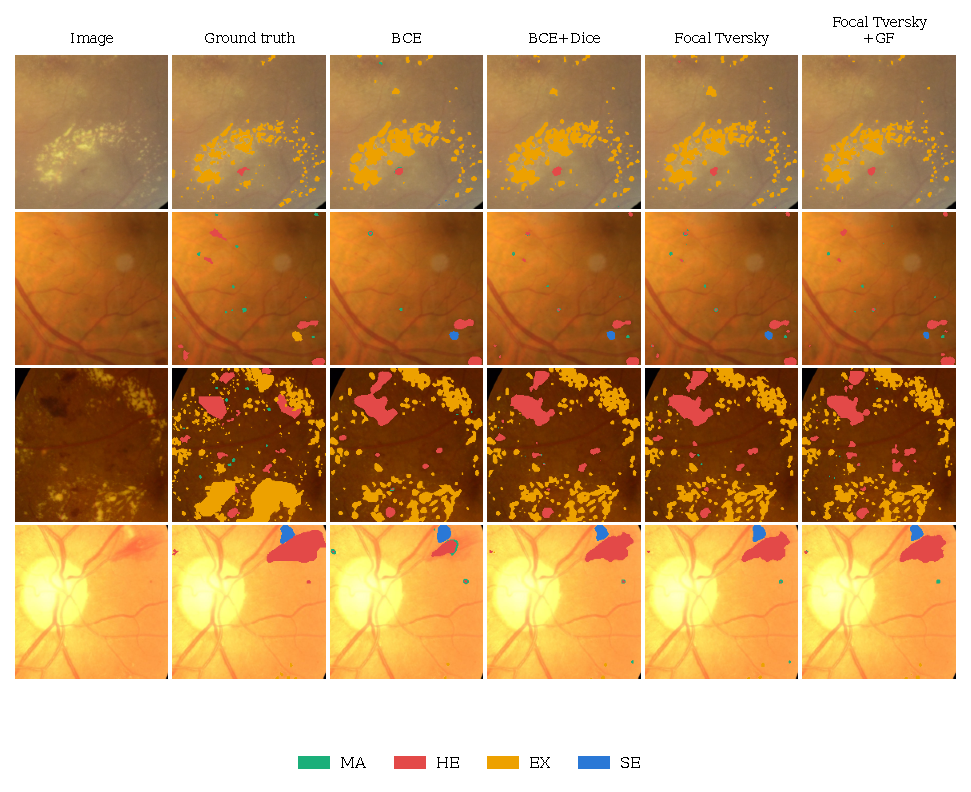
\includegraphics[width=.95\textwidth]{fig_seg_qual.pdf}
\caption{Qualitative segmentation results on four DDR test images (crops of $192\times192$ pixels containing many lesions), with predictions thresholded at each model's validation-optimal threshold. Columns: input, ground truth, and the four U-Net variants. Colours: MA green, HE red, EX yellow, SE blue.}
\label{fig:seg-qual}
\end{figure}

\begin{figure}[!htbp]
\centering
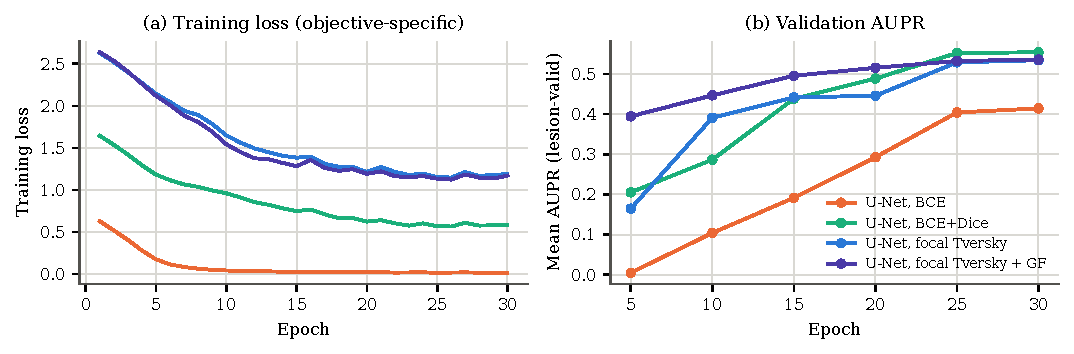
\includegraphics[width=\textwidth]{fig_seg_curves.pdf}
\caption{Segmentation training. (a) Training loss (objectives differ in scale and are not comparable across methods). (b) Mean AUPR over the four lesion classes on the lesion-validation split at the evaluation epochs.}
\label{fig:seg-curves}
\end{figure}

\begin{figure}[!htbp]
\centering
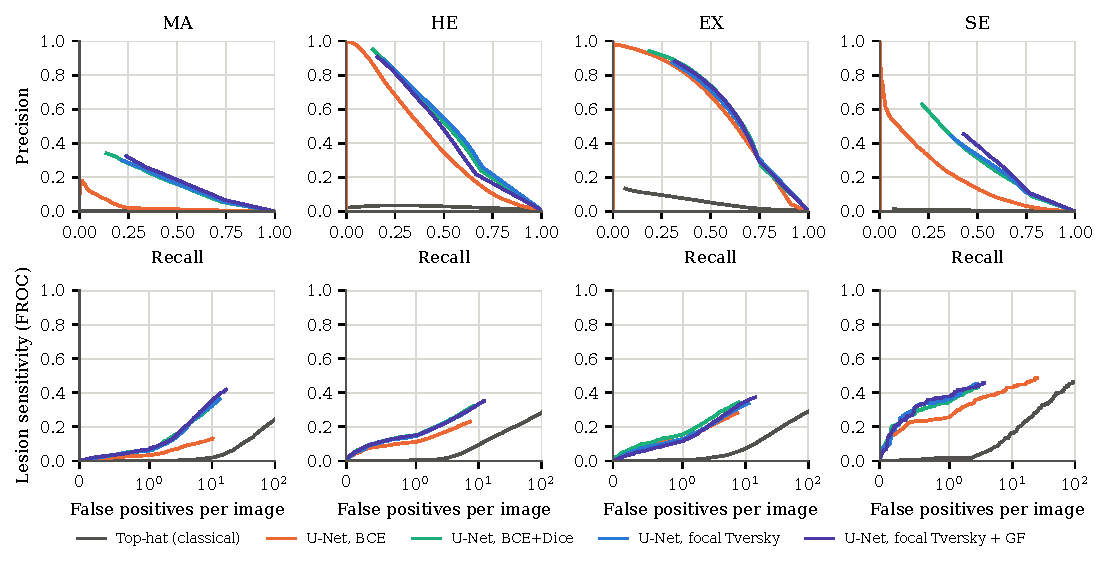
\includegraphics[width=\textwidth]{fig_froc_pr.pdf}
\caption{Per-class precision--recall curves of pixel probabilities (top) and lesion-level FROC curves of segmentation-derived detections (bottom; false positives per image on a symmetric-log axis), DDR test split.}
\label{fig:froc-pr}
\end{figure}

\subsection{Lesion detection}
\label{sec:res-det}
Tables~\ref{tab:det} and~\ref{tab:froc} report the detections obtained from the segmentation maps (Alg.~\ref{alg:det}), and Fig.~\ref{fig:det-qual} shows examples.

\paragraph{Overall level} Detection through connected-component proposals is weak at the standard IoU of 0.5, and moderate at relaxed overlap. The mean AP at IoU 0.3 is \nDetMapFtlbg\ for the GF variant (\nDetMapFtl\ raw; \nDetMapBcedice\ BCE+Dice; \nDetMapBce\ BCE; \nDetMapMorph\ for the classical baseline). At IoU 0.5 the AP of micro-aneurysms is below 0.01: a box that is one or two pixels off in each direction already drops below the threshold, which is a property of the metric on tiny objects more than of the detector, and the AP of haemorrhages and exudates is 0.06--0.08. Soft exudates reach AP$_{0.5}$ of 0.155--0.168, in line with their larger size but with only 214 test boxes the estimate is noisy.

\paragraph{FROC} At 8 false positives per image, the sensitivities of the best models are about 0.29--0.32 for microaneurysms, 0.31--0.32 for haemorrhages, 0.31--0.34 for exudates and 0.43--0.46 for soft exudates (Table~\ref{tab:froc}); they saturate at 16 false positives per image (0.32--0.41), which reflects that lesions missed by the segmentation (and therefore never proposed) bound the recall. The ordering of segmentation variants is the same as in segmentation: the plain cross-entropy model is clearly worse (mAP$_{0.3}$ 0.109) and the other three are close (0.161--0.168).

\paragraph{Why detection is hard here} Several factors explain the low numbers: (i) very high lesion density (the test images have 76 boxes on average), so adjacent lesions merge into one connected component; (ii) boxes of the order of 10 pixels or less; (iii) annotation boxes derived from pixel masks, which are not independent of segmentation errors; and (iv) the use of a seed threshold selected on validation AP$_{0.3}$ (the selected seeds differ widely between classes, 0.05--0.71, indicating that the probability maps are not calibrated across classes). We did not train a dedicated detector (Section~\ref{sec:setup}), so we cannot say how this approach compares with Faster R-CNN or FCOS; the value of the segmentation-derived route is that it requires no additional training and shares weights with the other tasks.

\begin{table}[!htbp]
\centering
\caption{Lesion detection on the DDR test split from segmentation-derived proposals (Alg.~\ref{alg:det}). AP$_{0.5}$ / AP$_{0.3}$ are average precision at IoU 0.5 / 0.3; the last column is the mean of AP$_{0.3}$ over the four classes. The ground truth contains 2041 MA, 6457 HE, 8320 EX and 214 SE boxes.}
\label{tab:det}
\small
\setlength{\tabcolsep}{3.5pt}
\begin{tabular}{@{}lcccccccc|c@{}}
\toprule
 & \multicolumn{2}{c}{MA} & \multicolumn{2}{c}{HE} & \multicolumn{2}{c}{EX} & \multicolumn{2}{c|}{SE} & \\
Proposals from & AP$_{.5}$ & AP$_{.3}$ & AP$_{.5}$ & AP$_{.3}$ & AP$_{.5}$ & AP$_{.3}$ & AP$_{.5}$ & AP$_{.3}$ & mAP$_{.3}$ \\
\midrule
Top-hat + threshold (classical) & 0.000 & 0.002 & 0.006 & 0.023 & 0.015 & 0.038 & 0.002 & 0.004 & 0.017 \\
U-Net, focal Tversky (ours) & 0.009 & 0.078 & 0.080 & 0.178 & 0.059 & 0.189 & 0.172 & 0.203 & 0.162 \\
U-Net, focal Tversky, GF input (ours) & 0.008 & 0.088 & 0.080 & 0.176 & 0.064 & 0.201 & 0.166 & 0.197 & \textbf{0.165} \\
\bottomrule
\end{tabular}
\end{table}

\begin{table}[!htbp]
\centering
\caption{Lesion-level FROC sensitivity of segmentation-derived detections (a prediction is a hit if its centre lies inside a ground-truth box) at 1, 2, 4, 8 and 16 false positives per image (FP/img), DDR test split.}
\label{tab:froc}
\small
\resizebox{\textwidth}{!}{%
\begin{tabular}{@{}llccccc@{}}
\toprule
Proposals from & Class & 1 & 2 & 4 & 8 & 16 \\
\midrule
Top-hat + threshold (classical) & MA & 0.000 & 0.001 & 0.004 & 0.014 & 0.040 \\
 & HE & 0.003 & 0.007 & 0.028 & 0.076 & 0.135 \\
 & EX & 0.004 & 0.011 & 0.027 & 0.058 & 0.113 \\
 & SE & 0.019 & 0.019 & 0.056 & 0.136 & 0.234 \\
\addlinespace
U-Net, BCE & MA & 0.032 & 0.056 & 0.090 & 0.119 & 0.131 \\
 & HE & 0.111 & 0.147 & 0.188 & 0.229 & 0.229 \\
 & EX & 0.128 & 0.178 & 0.233 & 0.282 & 0.282 \\
 & SE & 0.257 & 0.332 & 0.379 & 0.421 & 0.449 \\
\addlinespace
U-Net, focal Tversky, GF input & MA & 0.067 & 0.115 & 0.209 & 0.319 & 0.412 \\
 & HE & 0.150 & 0.194 & 0.250 & 0.309 & 0.351 \\
 & EX & 0.115 & 0.178 & 0.254 & 0.330 & 0.373 \\
 & SE & 0.379 & 0.425 & 0.458 & 0.458 & 0.458 \\
\addlinespace
\bottomrule
\end{tabular}}
\end{table}


\begin{figure}[!htbp]
\centering
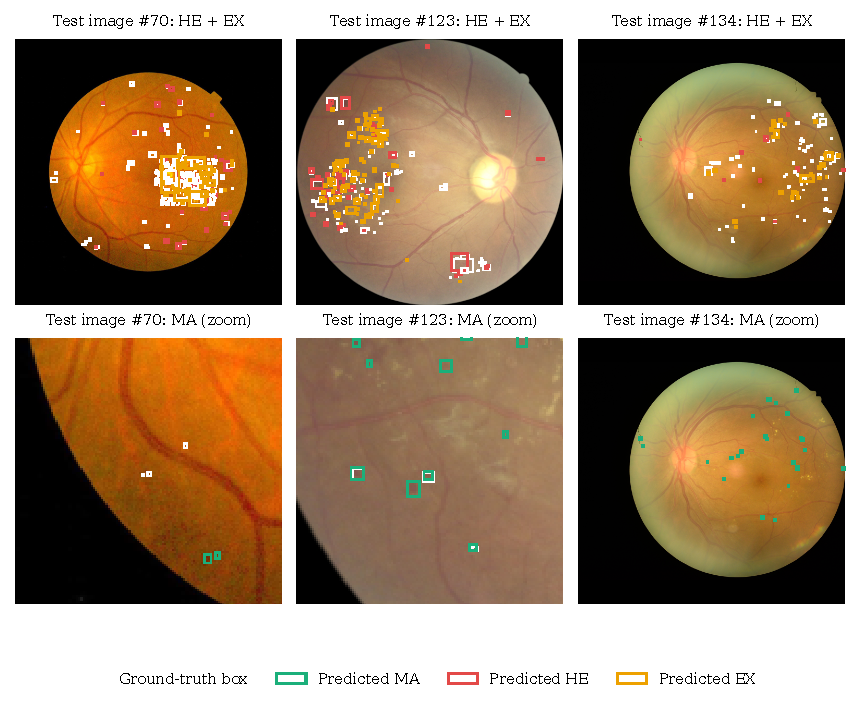
\includegraphics[width=.9\textwidth]{fig_det_qual.pdf}
\caption{Segmentation-derived detections (GF model) on three DDR test images: ground-truth boxes (white) and predicted boxes (HE red, EX yellow, MA green; predictions with low score are hidden for legibility). Top: haemorrhages and exudates; bottom: microaneurysms in a magnified region.}
\label{fig:det-qual}
\end{figure}

\subsection{What the lesion maps look like, and how lesion evidence relates to grade}
\label{sec:res-evidence}
Fig.~\ref{fig:example-maps} shows the lesion maps predicted for one random test image per grade. Maps are almost empty for grade~0, contain scattered microaneurysm and exudate responses for grades~1--2, and become dense and multi-class for the higher grades. The grade-4 example also illustrates a failure mode: a large pre-retinal structure in this image attracts haemorrhage and exudate responses over a wide area, which is not a ``lesion count'' in the clinical sense (the aggregated statistics would overstate the burden). Because the maps are summarised into the evidence tensor $Z$, we can also look at the statistics directly. Fig.~\ref{fig:evidence} shows, for each lesion class and zone, the mean $\log(1+n^{(0.5)})$ over the test images of each true grade. The soft counts of haemorrhages, hard exudates and soft exudates are clearly higher for grades~2--4 than for grades~0--1 in every zone, with the largest differences in the whole-field and quadrant statistics, and are not strictly monotone between the highest grades; the central-disc statistic is smaller than the others. Microaneurysm evidence is the least discriminative class (its mean varies little with grade), consistent with its weak segmentation quality (Section~\ref{sec:res-seg}). The statistics therefore carry the signal that the rules (Eqs.~\ref{eq:r1}--\ref{eq:r4}) rely on, but they are noisy at individual-image level.

\begin{figure}[!htbp]
\centering
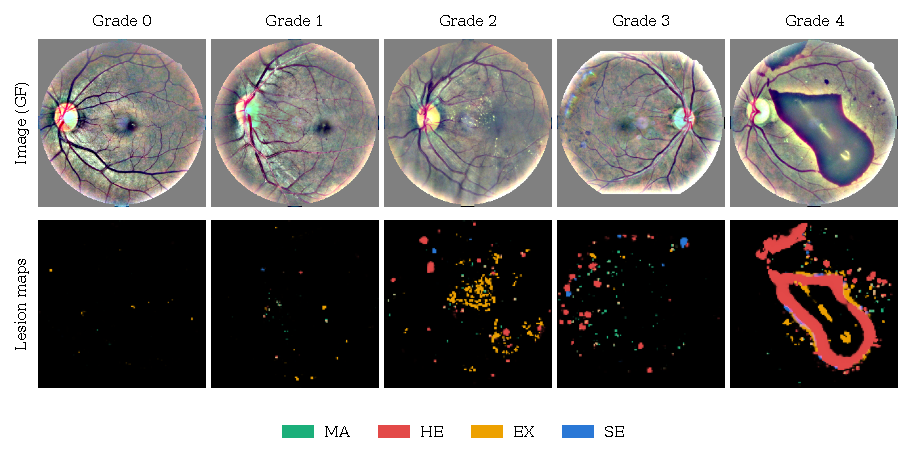
\includegraphics[width=\textwidth]{fig_example_maps.pdf}
\caption{Gaussian-filtered inputs (top) and predicted lesion probability maps (bottom, $128\times128$ after max-pooling, colour = class as in Fig.~\ref{fig:ddr-lesions}) for one randomly chosen test image of each grade. The grade-4 image shows a large non-lesion structure producing wide responses.}
\label{fig:example-maps}
\end{figure}

\begin{figure}[!htbp]
\centering
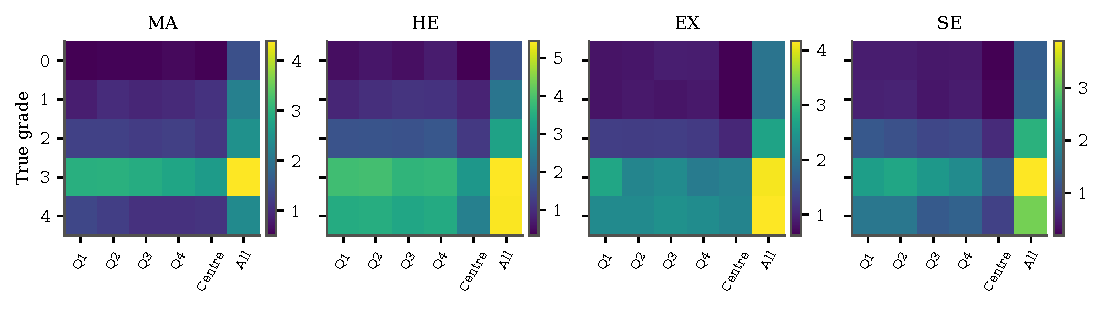
\includegraphics[width=\textwidth]{fig_evidence.pdf}
\caption{Mean zone-wise lesion evidence $\log(1+n^{(0.5)}_{c,z})$ by true grade (rows) and zone (columns: four quadrants Q1--Q4, central disc, whole field) on the leak-controlled test set, one panel per lesion class.}
\label{fig:evidence}
\end{figure}

\subsection{Grading performance}
\label{sec:res-grading}
Table~\ref{tab:grading} and Fig.~\ref{fig:ablation} report the five-class grading results. We discuss four findings in turn.

\paragraph{(1) Lesion evidence improves grading substantially.} The two models that use only the frozen image embedding (B1, B2) reach a QWK of \nBoneQWK\ and \nBtwoQWK. A model that sees \emph{only} the 120-dimensional evidence tensor (B3) reaches the same agreement (0.641) with 0.016\,M instead of 0.30\,M parameters, which says that the lesion maps contain as much grading information as a generic 1152-dimensional ImageNet embedding. Combining the two is clearly better than either alone: the naive concatenation B4 reaches 0.722, and \mname\ reaches \nMainQWK\ ($\pm\,\nMainQWKsd$ over five seeds; 95\% bootstrap interval [\nMainCIlo, \nMainCIhi]). The paired bootstrap difference between \mname\ and B1/B2/B3 is $+0.087/+0.095/+0.092$ with intervals that exclude zero by a wide margin (Table~\ref{tab:grading}). The AUC for referable DR rises from 0.865--0.867 (B1, B2) to \nMainAUC. Ablation A1, which keeps everything except the evidence tokens in the head, falls back to 0.632, i.e. to the level of B2 and \emph{not} to that of the full model, which shows that the gain comes from the evidence \emph{as input} to the head, not from the soft labels or the rule loss alone.

\paragraph{(2) Evidence tokens versus naive concatenation: a small gain.} The token-based head is better than concatenating the same inputs, but only slightly: the paired difference to B4 is $+0.013$ in QWK (95\% interval [0.001, 0.025]) and to the token head without soft labels or rule loss (T0) $+0.008$ ([0.000, 0.017]). With five seeds and a single backbone, we regard this as weak evidence that the token structure helps beyond the information content of the evidence itself; its principal benefit, in our view, is interpretability (attention to $(c,z)$ tokens) rather than accuracy.

\paragraph{(3) Soft ordinal labels mainly improve calibration, not agreement.} Adding Gaussian-smoothed targets (T1) changes QWK by $+0.010$ relative to T0 (seed-level SDs are 0.014), i.e. not reliably, but it reduces the expected calibration error from 0.095 to 0.058 (and to \nMainECE\ for the full model, versus \nBoneECE\ for B1 and \nBtwoECE\ for B2). This is consistent with the intended role of the soft target: it prevents the cumulative logits from saturating when adjacent grades are confused.

\paragraph{(4) The rule loss gives no measurable accuracy gain on DDR.} T2 (rule loss, no soft labels) scores 0.729 versus 0.722 for T0, and the full model is within 0.001 of T1 (paired difference +0.001, interval [$-$0.008, 0.010]). The reason is visible in Section~\ref{sec:res-rule}: grade predictions of \emph{all} models are already consistent with the fitted rules in more than 94\% of cases, so there is little left to correct.

\paragraph{Per-class behaviour.} Fig.~\ref{fig:grading}a shows where the errors are. Grade~0 is recognised with recall 0.98, and moderate (0.58) and proliferative DR (0.58) with precision around 0.75--0.78. Mild DR (grade~1) and severe NPDR (grade~3) are the weak classes (recall 0.04 and 0.07; F1 0.06 and 0.12): grade~1 is mostly predicted as grade~0 or~2, and grade~3 as grade~2 or~4. These are the two rarest classes (1.7\% and 4.6\% of training images for grades 3 and 1, respectively) and are defined by fine distinctions (a few microaneurysms; the 4--2--1 rule), so a low macro-F1 (\num{0.46}) is unsurprising, but it is a clear limitation. Overall, 82.5\% of the predictions are within one grade of the label, and the dominant error mode is the confusion of grade~2 with grade~0 (37\% of grade-2 images are called normal). On the six-class protocol (Table~\ref{tab:six}) accuracy is 0.734 for \mname\ versus 0.692 (B1); the quality gate separates ungradable from gradable images with AUC 0.995 for every model.

\begin{table}[!htbp]
\centering
\caption{Per-class results of \mname\ on the leak-controlled test set (seed-averaged probabilities, 3633 images).}
\label{tab:perclass}
\small
\begin{tabular}{@{}lccccc@{}}
\toprule
 & G0 & G1 & G2 & G3 & G4 \\
\midrule
Support & 1880 & 163 & 1265 & 61 & 264 \\
Precision & 0.77 & 0.12 & 0.75 & 0.67 & 0.78 \\
Recall & 0.98 & 0.04 & 0.58 & 0.07 & 0.58 \\
F1 & 0.86 & 0.06 & 0.66 & 0.12 & 0.66 \\
\bottomrule
\end{tabular}
\end{table}

\begin{table}[!htbp]
\centering
\caption{Five-class DR grading on the leak-controlled DDR test set (3633 gradable images), mean $\pm$ SD over 5 seeds. QWK 95\% CI: bootstrap over test images of the seed-averaged probabilities. $\Delta$QWK: paired bootstrap difference (\mname\ minus model), with 95\% interval; intervals excluding 0 are marked $^{*}$. Rule viol.: fraction of test images whose predicted grade is not licensed by the frozen rule scores (Section~\ref{sec:rule}).}
\label{tab:grading}
\footnotesize
\setlength{\tabcolsep}{2.8pt}
\resizebox{\textwidth}{!}{%
\begin{tabular}{@{}lcccccccc@{}}
\toprule
Model & QWK & 95\% CI & Acc. & F1 & AUC$_{\ge2}$ & ECE & Rule viol. & $\Delta$QWK \\
\midrule
B1: embedding, CE & 0.644$\pm$0.009 & [0.623, 0.669] & 0.686$\pm$0.006 & 0.439$\pm$0.011 & 0.865$\pm$0.003 & 0.093$\pm$0.008 & 0.046$\pm$0.004 & +0.087 [+0.071, +0.103]$^{*}$ \\
B2: embedding, ordinal & 0.638$\pm$0.010 & [0.616, 0.662] & 0.683$\pm$0.005 & 0.428$\pm$0.008 & 0.867$\pm$0.005 & 0.120$\pm$0.010 & 0.044$\pm$0.005 & +0.095 [+0.079, +0.111]$^{*}$ \\
B3: evidence only & 0.641$\pm$0.003 & [0.619, 0.665] & 0.697$\pm$0.005 & 0.449$\pm$0.007 & 0.877$\pm$0.002 & 0.047$\pm$0.005 & 0.039$\pm$0.008 & +0.092 [+0.072, +0.112]$^{*}$ \\
B4: embedding + evidence (concat.) & 0.722$\pm$0.011 & [0.702, 0.741] & 0.738$\pm$0.007 & 0.486$\pm$0.007 & 0.920$\pm$0.003 & 0.089$\pm$0.011 & 0.049$\pm$0.004 & +0.013 [+0.001, +0.025]$^{*}$ \\
T0: evidence tokens & 0.722$\pm$0.014 & [0.706, 0.747] & 0.748$\pm$0.010 & 0.454$\pm$0.017 & 0.921$\pm$0.004 & 0.095$\pm$0.015 & 0.052$\pm$0.005 & +0.008 [+0.000, +0.017]$^{*}$ \\
T1: T0 + soft labels & 0.732$\pm$0.014 & [0.714, 0.753] & 0.745$\pm$0.007 & 0.472$\pm$0.022 & 0.923$\pm$0.002 & 0.058$\pm$0.014 & 0.051$\pm$0.007 & +0.001 [-0.008, +0.010] \\
T2: T0 + rule loss & 0.729$\pm$0.017 & [0.714, 0.753] & 0.745$\pm$0.008 & 0.457$\pm$0.025 & 0.921$\pm$0.005 & 0.090$\pm$0.012 & 0.044$\pm$0.008 & +0.001 [-0.007, +0.009] \\
\textbf{\mname\ (full)} & 0.734$\pm$0.009 & [0.714, 0.754] & 0.745$\pm$0.011 & 0.464$\pm$0.018 & 0.923$\pm$0.004 & 0.057$\pm$0.003 & 0.045$\pm$0.008 & -- \\
A1: \mname\ w/o evidence tokens & 0.632$\pm$0.015 & [0.618, 0.664] & 0.682$\pm$0.003 & 0.408$\pm$0.017 & 0.851$\pm$0.006 & 0.088$\pm$0.009 & 0.041$\pm$0.008 & +0.093 [+0.077, +0.109]$^{*}$ \\
\bottomrule
\end{tabular}}
\end{table}

\begin{table}[!htbp]
\centering
\caption{Six-class protocol (ungradable images included) on the leak-controlled test set: a separate quality gate decides ``ungradable; otherwise the ordinal grade is output. Mean $\pm$ SD over 5 seeds.}
\label{tab:six}
\small
\begin{tabular}{@{}lccc@{}}
\toprule
Model & Accuracy & Macro-F1 & Gate AUC \\
\midrule
B1: embedding, CE & 0.692$\pm$0.005 & 0.488$\pm$0.012 & 0.995$\pm$0.000 \\
B2: embedding, ordinal & 0.676$\pm$0.004 & 0.495$\pm$0.007 & 0.995$\pm$0.000 \\
B3: evidence only & 0.678$\pm$0.006 & 0.505$\pm$0.004 & 0.995$\pm$0.000 \\
B4: embedding + evidence (concat.) & 0.726$\pm$0.006 & 0.543$\pm$0.006 & 0.995$\pm$0.000 \\
T0: evidence tokens & 0.736$\pm$0.007 & 0.530$\pm$0.012 & 0.995$\pm$0.000 \\
T1: T0 + soft labels & 0.735$\pm$0.007 & 0.532$\pm$0.011 & 0.995$\pm$0.000 \\
T2: T0 + rule loss & 0.733$\pm$0.008 & 0.538$\pm$0.016 & 0.995$\pm$0.000 \\
\textbf{\mname\ (full)} & 0.734$\pm$0.010 & 0.533$\pm$0.010 & 0.995$\pm$0.000 \\
A1: \mname\ w/o evidence tokens & 0.669$\pm$0.003 & 0.482$\pm$0.011 & 0.995$\pm$0.000 \\
\bottomrule
\end{tabular}
\end{table}


\begin{figure}[!htbp]
\centering
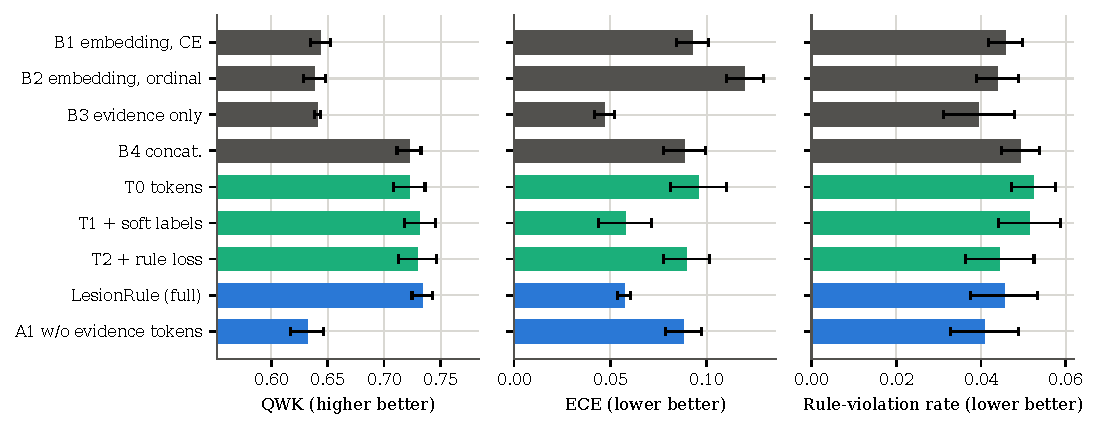
\includegraphics[width=\textwidth]{fig_ablation.pdf}
\caption{Grading models of Table~\ref{tab:methods} (mean $\pm$ SD over five seeds): quadratic-weighted kappa, expected calibration error and rule-violation rate. Grey: baselines using the embedding and/or evidence in simple form; green: evidence-token models; blue: full \mname\ and the ablation without evidence tokens (A1).}
\label{fig:ablation}
\end{figure}

\begin{figure}[!htbp]
\centering
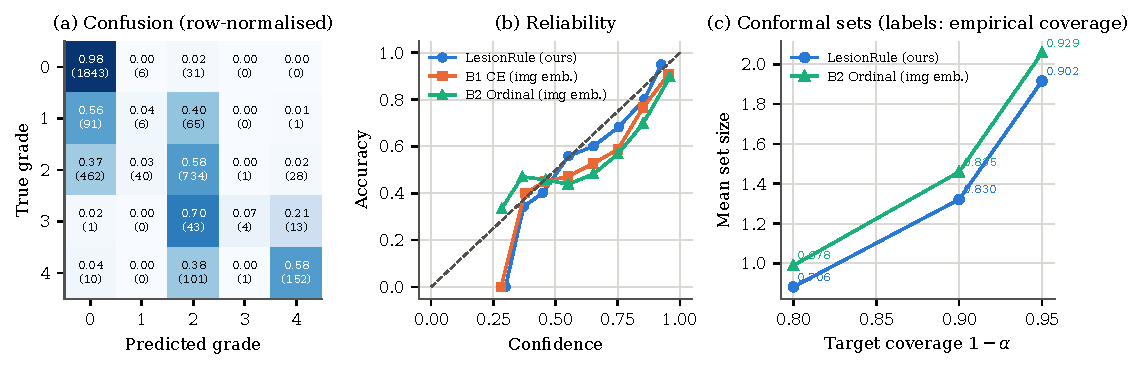
\includegraphics[width=\textwidth]{fig_grading.pdf}
\caption{(a) Row-normalised confusion matrix of \mname\ with counts. (b) Reliability diagram (10 bins) for \mname\ and two baselines. (c) Mean conformal set size against target coverage (calibration on the validation partition); numbers give the empirical coverage on the test set, which is below the target (Section~\ref{sec:res-conf}).}
\label{fig:grading}
\end{figure}

\subsection{Rule consistency}
\label{sec:res-rule}
Under the frozen rule scores, the fraction of test predictions that exceed what the lesion evidence licenses is 3.9--5.2\% for all models (Table~\ref{tab:grading}; Fig.~\ref{fig:ablation}, right). The full model has \nMainViol\% and the model without lesion evidence in the head, B2, has \nBtwoViol\%; the token model without rule loss (T0) has the highest rate (5.2\%) and the rule-loss variants (T2, full) are 0.7--0.8 percentage points lower, a small shift that is of the same order as the seed-to-seed spread (SD up to 0.8 points). We therefore cannot claim that the rule-consistency loss reduces contradictions in a meaningful way on this data. Two explanations are consistent with the numbers. First, the rules were calibrated on the training labels as necessary conditions (Eq.~\ref{eq:rulefit}), so they are permissive by construction: the threshold of each rule settles where it is hardly ever violated by true labels, and because every model has learned this association from the same evidence, very few predictions fall outside it. Second, the weakest classes (mild and severe) are rarely predicted, which removes many opportunities to violate rules defined for $y\ge1$ and $y\ge3$. Stricter, anatomically defined rules (Section~\ref{sec:limits}) or hand-specified thresholds would be needed to test the idea properly.

\subsection{Calibration and conformal referral}
\label{sec:res-conf}
\paragraph{Calibration.} After temperature scaling on validation half~A, the ECE of the full model is \nMainECE, versus \nBoneECE\ for the cross-entropy MLP and \nBtwoECE\ for the ordinal MLP (Fig.~\ref{fig:grading}b). The reliability curves lie close to the diagonal for confidence above 0.5, with the largest deviations in sparsely populated low-confidence bins.

\paragraph{Conformal sets calibrated on the DDR validation partition.} Table~\ref{tab:conformal} shows that the conformal sets calibrated on validation half~B \emph{do not} reach the nominal coverage on the test set: with $\alpha=0.05$, 0.1 and 0.2 the empirical coverage of \mname\ is \nConfCovFive, \nConfCovTen\ and \nConfCovTwenty\ (targets 0.95, 0.90, 0.80), and the other models behave similarly. This is not a failure of the method but of its assumption: the DDR validation and test partitions are \emph{not exchangeable}. Table~\ref{tab:shift} shows that the same model reaches an accuracy of \nValBAcc\% on validation half~B but \nTestAcc\% on the test set, although the class proportions are practically identical (e.g.\ 51\% versus 52\% grade~0), with similar differences in QWK and log-loss. The nonconformity scores of the calibration set are therefore systematically smaller than those of the test set, and the quantile is too optimistic. We could not determine the origin of this shift (the dataset documentation does not describe how the partitions were formed; differences in hospital, camera or annotation batch are plausible).

\paragraph{Conformal sets under exchangeability.} To verify that the construction itself works, Table~\ref{tab:conf-exch} calibrates on a random half of the test set and evaluates on the other half (300 random splits). Coverage is then 0.950, \nExchCovTen\ and 0.800 at the three nominal levels, with a standard deviation of about 0.01, as the theory (Appendix~\ref{app:proofs}) predicts. In this setting the referral rule (``refer if the set contains any grade $\ge2$'') at $\alpha=0.1$ achieves a sensitivity of 0.845 and a specificity of 0.876 for the lesion-grounded model, compared with 0.882 and 0.631 for the embedding-only ordinal model B2 (and 0.871/0.813 for concatenation B4), at similar mean set sizes (1.90 versus 1.84 and 1.64): the lesion evidence makes the model's \emph{uncertainty} more informative, so that fewer healthy patients are referred at a similar sensitivity. For comparison, simply taking the arg-max grade gives a referable-DR sensitivity of 0.677 and a specificity of 0.953 (B2: 0.538 and 0.951), i.e.\ hard decisions miss a large fraction of referable cases at this operating point, which is the practical argument for set-valued outputs. We emphasise that the exchangeable check used test labels for calibration and therefore describes what would happen with a calibration set drawn from the deployment distribution; it is not a test-set result in the usual sense.

\begin{table}[!htbp]
\centering
\caption{Split-conformal prediction sets (calibration: validation half B, 1252 images) evaluated on the leak-controlled test set. Coverage should be $\ge1-\alpha$. ``Refer = set contains any grade $\ge2$; sensitivity/specificity are for referable DR ($y\ge2$). Class-wise coverage shows that the guarantee is marginal.}
\label{tab:conformal}
\footnotesize
\setlength{\tabcolsep}{3pt}
\begin{tabular}{@{}llcccccc@{}}
\toprule
Model & $\alpha$ & Coverage & Set size & Singleton & Refer sens. & Refer spec. & Cov. G0/G1/G2/G3/G4 \\
\midrule
\textbf{\mname\ (full)} & 0.05 & 0.902 & 1.92 & 0.34 & 0.849 & 0.874 & 0.99/0.92/0.80/0.80/0.74 \\
 & 0.1 & 0.830 & 1.32 & 0.75 & 0.767 & 0.922 & 0.99/0.44/0.70/0.43/0.65 \\
 & 0.2 & 0.706 & 0.88 & 0.88 & 0.560 & 0.971 & 0.97/0.00/0.48/0.00/0.51 \\
\addlinespace
B1: embedding, CE & 0.05 & 0.915 & 1.96 & 0.35 & 0.906 & 0.574 & 1.00/0.38/0.88/0.69/0.87 \\
 & 0.1 & 0.829 & 1.43 & 0.63 & 0.771 & 0.798 & 1.00/0.10/0.71/0.46/0.75 \\
 & 0.2 & 0.679 & 0.98 & 0.95 & 0.514 & 0.944 & 0.97/0.00/0.38/0.13/0.58 \\
\addlinespace
B2: embedding, ordinal & 0.05 & 0.929 & 2.06 & 0.34 & 0.925 & 0.535 & 1.00/0.49/0.91/0.75/0.86 \\
 & 0.1 & 0.835 & 1.46 & 0.62 & 0.782 & 0.784 & 1.00/0.10/0.72/0.61/0.73 \\
 & 0.2 & 0.678 & 0.99 & 0.96 & 0.512 & 0.947 & 0.98/0.00/0.38/0.11/0.53 \\
\addlinespace
B4: embedding + evidence (concat.) & 0.05 & 0.923 & 1.81 & 0.48 & 0.899 & 0.770 & 1.00/0.63/0.87/0.77/0.85 \\
 & 0.1 & 0.838 & 1.30 & 0.74 & 0.795 & 0.900 & 1.00/0.17/0.73/0.52/0.73 \\
 & 0.2 & 0.709 & 0.93 & 0.93 & 0.577 & 0.960 & 0.98/0.01/0.46/0.18/0.51 \\
\addlinespace
\bottomrule
\end{tabular}
\end{table}

\begin{table}[!htbp]
\centering
\caption{Conformal coverage under exchangeability: the leak-controlled test set is split at random into a calibration half and an evaluation half (300 repetitions; mean $\pm$ SD). Compare with Table~\ref{tab:conformal}, where calibration used the DDR validation partition. ``Refer = set contains any grade $\ge2$.}
\label{tab:conf-exch}
\small
\resizebox{\textwidth}{!}{%
\begin{tabular}{@{}llcccc@{}}
\toprule
Model & $\alpha$ & Coverage & Set size & Refer sens. & Refer spec. \\
\midrule
\textbf{\mname\ (full)} & 0.05 & 0.950$\pm$0.008 & 2.75 & 0.913 & 0.770 \\
 & 0.1 & 0.900$\pm$0.011 & 1.90 & 0.845 & 0.876 \\
 & 0.2 & 0.800$\pm$0.014 & 1.17 & 0.733 & 0.936 \\
\addlinespace
B2: embedding, ordinal & 0.05 & 0.950$\pm$0.007 & 2.29 & 0.952 & 0.444 \\
 & 0.1 & 0.900$\pm$0.010 & 1.84 & 0.882 & 0.631 \\
 & 0.2 & 0.799$\pm$0.013 & 1.33 & 0.726 & 0.839 \\
\addlinespace
B4: embedding + evidence (concat.) & 0.05 & 0.950$\pm$0.007 & 2.10 & 0.934 & 0.676 \\
 & 0.1 & 0.899$\pm$0.010 & 1.64 & 0.871 & 0.813 \\
 & 0.2 & 0.800$\pm$0.013 & 1.17 & 0.745 & 0.920 \\
\addlinespace
\bottomrule
\end{tabular}}
\end{table}

\begin{table}[!htbp]
\centering
\caption{Partition shift inside DDR: the same models evaluated on validation half B (the conformal calibration set, 1252 images) and on the leak-controlled test set (3633 images), seed-averaged probabilities. Class proportions are practically identical in the two sets.}
\label{tab:shift}
\small
\begin{tabular}{@{}lcccc@{}}
\toprule
Model & Acc. (val B) & Acc. (test) & QWK (val B) & QWK (test) \\
\midrule
\textbf{\mname\ (full)} & 0.839 & 0.754 & 0.857 & 0.735 \\
B2: embedding, ordinal & 0.802 & 0.685 & 0.810 & 0.640 \\
\bottomrule
\end{tabular}
\end{table}


\subsection{Zero-shot external test}
\label{sec:res-ext}
Table~\ref{tab:external} gives the results of applying the DDR-trained heads to the Gaussian-filtered Kaggle set without adaptation. The transfer is poor for all models: QWK is between 0.10 and 0.23 and accuracy between 31\% and 50\% depending on the seed, with a large seed-to-seed variance (e.g.\ the QWK of the full model over the five seeds is 0.38, 0.27, 0.05, 0.28 and $-0.10$). The AUC for referable DR is 0.64--0.73, only moderately above chance. Inspection of the predictions shows that the models collapse onto grades~0 and~2: for the full model (seed 0), 41\% of the external images are predicted as grade~0, 59\% as grade~2 and essentially none as grades~1, 3 or~4, although the external set has 27\% grade-2 and 8\% grade-4 images. Three factors plausibly contribute: (i) the external images are $224\times224$, so microaneurysms and small haemorrhages are invisible and the lesion evidence is systematically underestimated; (ii) the segmentation network was trained on DDR images processed at full field of view and sees up-sampled, already-filtered inputs; (iii) the populations and cameras differ. The model with the rule loss and no soft labels (T2) has the highest mean QWK (0.227) and B2 reaches 0.215, but with five seeds and these standard deviations no ranking of models is supported. We report this negative result because it bounds the claims of the paper: \emph{within DDR}, lesion evidence adds clearly to the embedding; \emph{across datasets}, our pipeline does not generalise at this resolution, and the conformal guarantee could not be expected to hold either.

\begin{table}[!htbp]
\centering
\caption{Zero-shot external test on the Gaussian-filtered APTOS-derived Kaggle set (3664 images, $224\times224$, grades 0--4): models trained on DDR only, no adaptation (mean $\pm$ SD over 5 seeds). Lesion evidence is computed by the segmentation network applied to the up-sampled images.}
\label{tab:external}
\small
\begin{tabular}{@{}lccccc@{}}
\toprule
Model & QWK & Acc. & F1 & AUC$_{\ge2}$ & Rule viol. \\
\midrule
B1: embedding, CE & 0.175$\pm$0.046 & 0.495$\pm$0.030 & 0.219$\pm$0.016 & 0.680$\pm$0.037 & 0.018$\pm$0.007 \\
B2: embedding, ordinal & 0.215$\pm$0.087 & 0.455$\pm$0.048 & 0.232$\pm$0.034 & 0.694$\pm$0.077 & 0.022$\pm$0.006 \\
B3: evidence only & 0.103$\pm$0.035 & 0.303$\pm$0.011 & 0.141$\pm$0.011 & 0.705$\pm$0.001 & 0.015$\pm$0.004 \\
B4: embedding + evidence (concat.) & 0.145$\pm$0.027 & 0.348$\pm$0.011 & 0.181$\pm$0.020 & 0.726$\pm$0.061 & 0.021$\pm$0.005 \\
T0: evidence tokens & 0.121$\pm$0.161 & 0.392$\pm$0.094 & 0.188$\pm$0.041 & 0.641$\pm$0.125 & 0.020$\pm$0.010 \\
T1: T0 + soft labels & 0.121$\pm$0.189 & 0.375$\pm$0.107 & 0.190$\pm$0.054 & 0.642$\pm$0.155 & 0.025$\pm$0.011 \\
T2: T0 + rule loss & 0.227$\pm$0.103 & 0.408$\pm$0.069 & 0.206$\pm$0.042 & 0.731$\pm$0.089 & 0.021$\pm$0.009 \\
\textbf{\mname\ (full)} & 0.176$\pm$0.174 & 0.381$\pm$0.079 & 0.199$\pm$0.035 & 0.657$\pm$0.147 & 0.022$\pm$0.011 \\
A1: \mname\ w/o evidence tokens & 0.172$\pm$0.111 & 0.452$\pm$0.066 & 0.215$\pm$0.039 & 0.648$\pm$0.052 & 0.023$\pm$0.010 \\
\bottomrule
\end{tabular}
\end{table}


\subsection{Which evidence matters? Zones and lesion classes}
\label{sec:res-evablate}
The design of the evidence bottleneck rests on two assumptions that the preceding results do not test: that resolving lesions by retinal zone helps, and that all four lesion classes contribute. Table~\ref{tab:evablate} answers both questions by training the full \mname\ head with parts of the evidence tensor set to zero (including in the rule scores), using three seeds.

\paragraph{Zones add little.} Restricting the evidence to the whole-field zone gives a QWK of 0.736, compared with 0.745 for the reference with all six zones (a difference of $-0.009$), and removing the whole-field zone but keeping the four quadrants and the central disc gives 0.733 ($-0.012$). With seed-level standard deviations of 0.007--0.022, neither difference can be distinguished from noise. On DDR, then, \emph{the global lesion statistics carry practically all of the evidence that the zone-wise statistics carry}; the zone resolution that motivated the token design (Section~\ref{sec:rationale}) is not shown to be beneficial. We see two explanations, which we cannot separate with the present data. The quadrants are image quadrants and not anatomically registered ETDRS fields, so they may not capture the spatial pattern that the clinical rules concern; and the grading label of DDR may depend mainly on the amount and type of lesions rather than on their spread, for example because the boundaries between the middle grades are drawn on counts. The result also means that our rule $R_3$, which uses quadrant-wise haemorrhage evidence, is less well supported than the other rules.

\paragraph{Lesion classes contribute unequally.} Removing haemorrhages costs 0.030 QWK, removing microaneurysms 0.024, removing soft exudates 0.019, and removing hard exudates only 0.004; the last difference is negligible although exudates are the best-segmented class (Section~\ref{sec:res-seg}), presumably because their information is redundant with the other classes and with the image embedding (large exudates are also visible to the ImageNet features). When a single class is kept, microaneurysm evidence reaches 0.704, haemorrhage evidence 0.687, soft-exudate evidence 0.674 and exudate evidence 0.630; the last is no better than the embedding-only models (0.638--0.644; Table~\ref{tab:grading}). It is striking that microaneurysms, the class with the lowest segmentation quality (AUPR at most 0.17), are the most informative \emph{single} class. A plausible reason is that microaneurysms are the earliest lesion and that ICDR grade~1 is defined by their presence alone, so that even a noisy microaneurysm signal separates grade~0 from higher grades. This implies that better microaneurysm segmentation, which requires higher-resolution input than we could afford, has the greatest potential to improve the grader. As with all ablations in this paper, these are three-seed estimates on a single backbone and should be read as indications.

\begin{table}[!htbp]
\centering
\caption{Evidence ablation: the full \mname\ head trained with parts of the evidence tensor removed (zones or lesion classes set to zero everywhere, including in the rule scores). Three seeds (0--2), mean $\pm$ SD, leak-controlled test set. $\Delta$ is the mean QWK difference to the reference. With three seeds and SDs of 0.005--0.02, differences below about 0.01 are not distinguishable from noise.}
\label{tab:evablate}
\small
\resizebox{\textwidth}{!}{%
\begin{tabular}{@{}lcccc@{}}
\toprule
Evidence kept & QWK & $\Delta$QWK & Acc. & ECE \\
\midrule
Full evidence (reference) & 0.745$\pm$0.007 & -- & 0.748$\pm$0.009 & 0.048$\pm$0.009 \\
Whole-field zone only & 0.736$\pm$0.013 & -0.008 & 0.747$\pm$0.013 & 0.056$\pm$0.012 \\
Quadrants + centre (no whole field) & 0.733$\pm$0.022 & -0.012 & 0.742$\pm$0.010 & 0.055$\pm$0.024 \\
Without MA & 0.721$\pm$0.002 & -0.023 & 0.739$\pm$0.000 & 0.055$\pm$0.002 \\
Without HE & 0.715$\pm$0.011 & -0.029 & 0.729$\pm$0.006 & 0.058$\pm$0.010 \\
Without EX & 0.741$\pm$0.011 & -0.003 & 0.747$\pm$0.003 & 0.054$\pm$0.021 \\
Without SE & 0.726$\pm$0.009 & -0.019 & 0.736$\pm$0.008 & 0.032$\pm$0.001 \\
MA only & 0.704$\pm$0.018 & -0.041 & 0.717$\pm$0.006 & 0.062$\pm$0.007 \\
HE only & 0.687$\pm$0.004 & -0.058 & 0.716$\pm$0.005 & 0.067$\pm$0.017 \\
EX only & 0.630$\pm$0.003 & -0.115 & 0.680$\pm$0.003 & 0.083$\pm$0.009 \\
SE only & 0.674$\pm$0.009 & -0.071 & 0.697$\pm$0.001 & 0.076$\pm$0.009 \\
\bottomrule
\end{tabular}}
\end{table}


\subsection{Failure analysis}
\label{sec:res-fail}
Fig.~\ref{fig:failures} shows, for the four most frequent error types of \mname, one of the 15 most confident wrong predictions (chosen at random among them with a fixed seed), together with its lesion maps. They illustrate failure modes that the aggregate numbers hide, and we describe them with the caveat that four images do not characterise a distribution.

\paragraph{Moderate called normal (37\% of grade-2 images).} The example has a confidence of 0.93 for ``normal'', and its lesion maps contain only a few scattered, low-intensity responses (a couple of microaneurysm and haemorrhage cells). In DDR, grade~2 can be assigned on the basis of microaneurysms and a few small haemorrhages, i.e.\ on lesions that are at or below the resolution of our segmentation network ($512^2$ for an image of about 2000 pixels). The confusion is therefore a direct consequence of the weakest component of the pipeline (microaneurysm and small-haemorrhage segmentation, Section~\ref{sec:res-seg}), and it explains why the largest class-wise gains are not to be expected from the grader but from higher-resolution lesion maps.

\paragraph{Normal called moderate.} The example (confidence 0.64) has many exudate responses scattered over the posterior pole. We cannot tell from the image alone whether these are real exudates that were not graded, drusen-like structures or reflection artefacts that the segmentation network mistook for exudates; since the DDR grades were assigned on the full-resolution photograph, each possibility is plausible. This example shows how the evidence-based design transmits segmentation errors directly to the grade, and why an uncertainty-aware output (conformal sets) is meant to help: a moderate-confidence prediction like this one is the situation in which a set with several grades is preferable to a single label.

\paragraph{Severe called moderate.} The grade~3 example has sparse lesion maps. The severe NPDR criteria rely on the extent of haemorrhages in four quadrants, venous beading and intraretinal microvascular abnormalities. Our evidence includes the first only through noisy haemorrhage maps, and has no representation of the other two. With only 61 test images of grade~3 and 118 in training, the head has few examples from which to learn the pattern, and recall is 0.07.

\paragraph{PDR called moderate.} Proliferative DR is defined by neovascularisation, vitreous or pre-retinal haemorrhage, none of which is a segmentation class in DDR. The example shows moderate-looking exudates and a few haemorrhages. This is a structural limitation of any model that uses only the four DDR lesion classes as evidence: the image embedding must provide the missing information, which in our frozen-backbone setting it does only partially (recall of grade~4: 0.58). A segmentation class for neovascularisation, or a fine-tuned backbone, is the natural remedy.

\begin{figure}[!htbp]
\centering
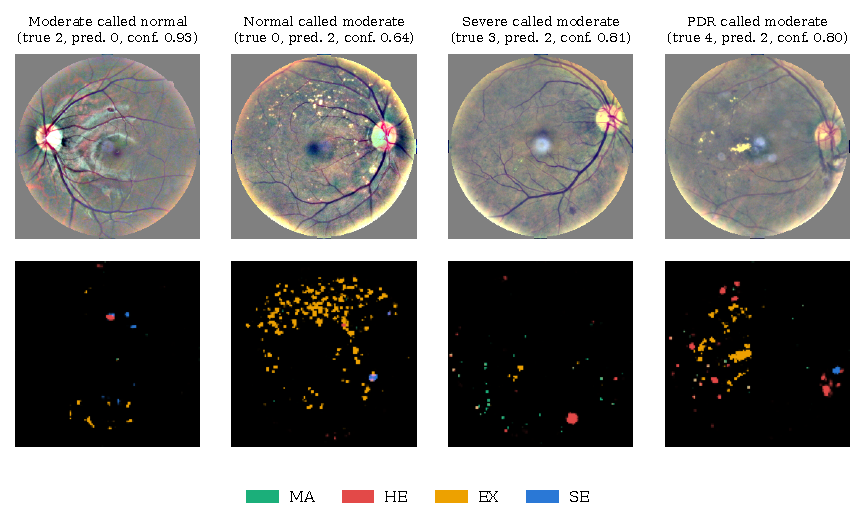
\includegraphics[width=\textwidth]{fig_failures.pdf}
\caption{Confidently wrong predictions of \mname\ on the leak-controlled test set (one example per error type, chosen at random among the 15 most confident errors of that type): Gaussian-filtered input (top) and lesion maps (bottom).}
\label{fig:failures}
\end{figure}

\subsection{End-to-end reference}
\label{sec:res-ft}
TO BE FILLED


\subsection{Computational cost}
\label{sec:res-cost}
Table~\ref{tab:cost} summarises measured costs on the four-core CPU machine. Training the segmentation network for 30 epochs takes about 23 minutes (45 seconds per epoch) with bfloat16 autocast; inference at $512\times512$ runs at about 0.12 seconds per image (8 images per second) for the network alone and about 3 images per second end-to-end, including decoding of the original 2-megapixel JPEG files, resizing and filtering, which is how the lesion maps for all \num{13673} DDR images were produced in roughly 75 minutes. The grading stage is negligible in comparison: the token head has 0.14\,M parameters and each of its training runs took a few minutes on a single core (while sharing the machine with other jobs), and evidence extraction for thousands of images takes seconds. The cost of \mname\ over the embedding-only baselines is therefore dominated by one segmentation pass per image. These timings are specific to this machine and are given to show that the whole study is reproducible without a GPU.

\begin{table}[!htbp]
\centering
\caption{Model sizes and measured costs (four CPU cores, bfloat16 autocast where applicable).}
\label{tab:cost}
\small
\begin{tabular}{@{}llrl@{}}
\toprule
Component & Role & Parameters & Measured cost \\
\midrule
U-Net (ResNet-18 + full-res branch) & lesion segmentation & 11.8\,M & train 23 min; 0.12 s/image at $512^2$ \\
ConvNeXt-T (frozen) & image embedding & 27.8\,M & feature extraction, 256$^2$ \\
MLP baselines (B1, B2, B4) & grading & 0.30\,M & seconds per run \\
Evidence MLP (B3) & grading & 0.016\,M & seconds per run \\
Evidence-token head (\mname) & grading & 0.14\,M & a few min per run (1 core) \\
\bottomrule
\end{tabular}
\end{table}

\section{Discussion}
\label{sec:discussion}
\subsection{Limitations}
\label{sec:limits}
We list the limitations that we consider material, from most to least consequential for the claims of this paper.

\paragraph{Compute-bound design} All experiments run on four CPU cores. The image embedding is a frozen ImageNet backbone, the segmentation network is trained at $512\times512$ on 383 images, and we could not train end-to-end grading networks at native resolution, large transformer backbones, retinal foundation models, or heavy detectors. Absolute grading accuracy is therefore lower than what a GPU-trained, fine-tuned system can reach, and the comparison with a fine-tuned ResNet-18 (Section~\ref{sec:res-ft}) is the only end-to-end reference we provide. The \emph{relative} conclusions (evidence tokens versus none, with versus without rule loss) are drawn under identical embeddings, but we cannot exclude that they change when the backbone is fine-tuned or replaced by a stronger one. This is the most important open question for follow-up work.

\paragraph{Single segmentation run} Segmentation and detection results come from one training run per configuration. Differences of a few thousandths between segmentation variants are within the range that seeds could change; we therefore base claims only on the larger differences, and we explicitly avoid significance statements for segmentation.

\paragraph{Train--test discrepancy in lesion evidence} The lesion maps of the 375 grading-training and validation images that are also lesion-training images (Appendix~\ref{app:leak}) are produced by a network that saw their pixel labels, and are therefore cleaner than those of unseen images. This slightly biases the evidence statistics seen during head training towards better lesion maps than at test time (about 4\% of the grading-training images). We removed the corresponding leak from the \emph{test} set, but did not re-train the segmenter on disjoint folds, which would be the cleaner solution.

\paragraph{Rule templates are surrogates} Neovascularisation, intraretinal microvascular abnormalities and venous beading are not annotated in DDR, so rules for severe and proliferative DR are only partial; the zones are image quadrants, not ETDRS fields defined with respect to the optic disc and fovea, because we did not localise those landmarks; and the thresholds are fitted on grade labels, which themselves contain noise. The rules should be read as clinically inspired regularisers and consistency checks, not as an implementation of the grading guideline, and a low violation rate does not by itself prove clinical correctness.

\paragraph{Conformal guarantee} The coverage guarantee is marginal, assumes exchangeability between calibration and test data, and does not hold under distribution shift or conditionally for rare grades (Section~\ref{sec:res-conf}). Because severe DR is rare, class-conditional coverage for grade~3 is estimated from few samples.

\paragraph{External validation} The only external test is a $224\times224$, Gaussian-filtered grading set without lesion annotations. It evaluates robustness of the grading pipeline to a shift in population, camera and resolution, but cannot validate lesion segmentation or detection, and it is not a substitute for prospective multi-centre validation. Conformal calibration was not re-done on the external set.

\paragraph{Labels and annotation} DDR grading labels carry inter-grader noise that we model only through soft ordinal targets. Training-set detection boxes contain duplicates (removed), the detection ground truth is derived from the same lesions as the masks and is therefore not an independent annotation, and microaneurysm annotation is known to be inconsistent. Resizing masks to $512\times512$ with a small area threshold preserves tiny lesions but also dilates some of them by a fraction of a pixel.

\paragraph{No clinical claim} The study is retrospective, on public data. It does not establish clinical utility, safety, or fairness across subgroups; DDR provides no demographic information, so subgroup performance could not be examined.

\subsection{Ethical considerations and responsible use}
Automated DR screening can extend access to care but can also cause harm when deployed without safeguards: false negatives delay treatment of sight-threatening disease, and systematic performance differences across populations, camera types and image quality can widen disparities. Three features of the proposed framework are meant to support responsible use, although none of them is sufficient on its own: lesion-grounded evidence tokens make the basis for a grade inspectable; the rule-violation rate flags internally inconsistent outputs; and conformal sets quantify when the model should abstain from a single-grade decision and refer the case to a human reader. The models and code are released for research only, in line with the non-commercial licence of DDR; any clinical use would require prospective validation, regulatory review, local calibration, and monitoring for distribution shift.

\subsection{Future work}
Four directions follow directly from the limitations. (i) \emph{End-to-end training}: because the evidence bottleneck is differentiable, the segmenter can be fine-tuned from grade supervision, and the fine-tuned image backbone can be replaced by a retinal foundation model \citep{zhou2023retfound}; this requires GPUs. (ii) \emph{Weak lesion supervision}: only 5.5\% of DDR images (757 of 13{,}673) have lesion annotations, but almost all have grades. A teacher--student scheme \citep{tarvainen2017meanteacher} with uncertainty gating \citep{gal2016dropout} and an attention-based multiple-instance loss \citep{ilse2018attentionmil} could use grades as weak lesion supervision; we implemented the building blocks (probability maps, evidence, rules) but did not run this experiment. (iii) \emph{Anatomical zones}: replacing quadrants by ETDRS fields registered to optic disc and fovea would make the rules closer to the clinical definition. (iv) \emph{Prospective and multi-centre evaluation} with conformal re-calibration under shift.


\section{Conclusion}
\label{sec:conclusion}
We studied DR grading, lesion segmentation and lesion detection as one coupled problem on the DDR dataset, with the grade computed from zone-wise soft lesion statistics of a segmentation network and complemented by ordinal soft targets, a clinical-rule consistency loss and conformal referral sets. Under a strictly controlled protocol --- a leak-controlled test set, five seeds, bootstrap intervals, matched baselines and component ablations --- the clearest finding is that lesion evidence adds information that a generic image embedding lacks: the quadratic-weighted kappa rises from 0.64 to 0.73 and the AUC for referable DR from 0.87 to 0.92, with a segmentation network trained on only 383 pixel-annotated images. Soft ordinal targets improve calibration; the token architecture gives a small gain over naive fusion; the rule-consistency loss did not change accuracy or violation rates measurably, because the rules are rarely violated to begin with. Conformal prediction delivers its guarantee under exchangeability but is not robust to the shift we found between the DDR validation and test partitions, and the pipeline does not transfer zero-shot to a low-resolution external set. Segmentation of small lesions (microaneurysms) and detection at strict overlap remain weak at the resolution that our compute allowed, and mild and severe DR are poorly recognised.

These conclusions come with the caveats of a CPU-bound, frozen-backbone study with single segmentation runs. The most valuable next steps are end-to-end fine-tuning with a stronger backbone, using grade labels as weak supervision for the 95\% of images without lesion masks, anatomically defined zones and stricter rules, and prospective multi-centre validation with calibration on the deployment distribution. We release code and every intermediate result so that these steps can be taken without re-running the CPU pipeline.

\section*{Declarations}
\paragraph{CRediT authorship contribution statement.} [To be completed by the authors.] Conceptualization, Methodology, Software, Validation, Formal analysis, Investigation, Data curation, Writing -- original draft, Writing -- review \& editing, Visualization, Supervision.

\paragraph{Declaration of competing interest.} [To be completed by the authors.] The authors declare that they have no known competing financial interests or personal relationships that could have appeared to influence the work reported in this paper.

\paragraph{Funding.} [To be completed by the authors.]

\paragraph{Data and code availability.} The DDR dataset is available from its authors at \url{https://github.com/nkicsl/DDR-dataset} (links to Google Drive and Baidu Drive; CC BY-NC-SA 4.0). The Gaussian-filtered Kaggle dataset is available at \url{https://www.kaggle.com/datasets/sovitrath/diabetic-retinopathy-224x224-gaussian-filtered} (CC0). Code, configuration files and result files that generate every table and figure in this paper are available in the repository \url{https://github.com/deep1789/Diabetic-Retinopathy}.

\paragraph{Declaration of generative AI and AI-assisted technologies in the writing process.} During the preparation of this work an AI assistant (Claude, Anthropic) was used to write code, run experiments and draft the manuscript text. The authors must review and edit all content and take full responsibility for the publication before submission. [Authors to confirm and adapt this statement according to the journal's policy.]

\paragraph{Ethics.} This study uses only publicly available, de-identified images; no new patient data were collected.


\appendix
\section{Overlap between lesion and grading partitions, and sensitivity analysis}
\label{app:leak}
Table~\ref{tab:overlap} shows how the 757 lesion-annotated images are distributed over the grading partitions, computed by matching file names. The two partitions are not aligned. The 126 grading-test images that also occur in the lesion-training (8) or lesion-validation (118) subsets are removed from the grading test set in all main experiments (leak-controlled test set, 3633 gradable images). Table~\ref{tab:sens} compares the main grading metrics on the leak-controlled and on the full official test partition (3759 gradable images).

\begin{table}[h]
\centering
\caption{Number of lesion-subset images (rows) found in each grading partition (columns), by file name.}
\label{tab:overlap}
\small
\begin{tabular}{@{}lrrrr@{}}
\toprule
Lesion subset & Grading train & Grading valid & Grading test & Total \\
\midrule
Lesion train (383) & 275 & 100 & 8 & 383 \\
Lesion valid (149) & 0 & 31 & 118 & 149 \\
Lesion test (225) & 152 & 12 & 59 & 223$^{*}$ \\
\bottomrule
\end{tabular}

\vspace{2pt}
{\footnotesize $^{*}$ Two lesion-test images are not listed in any grading partition.}
\end{table}

\begin{table}[h]
\centering
\caption{Sensitivity to the leak control: QWK (mean $\pm$ SD over 5 seeds) on the leak-controlled test set (3633 images) versus the full official gradable test partition (3759 images).}
\label{tab:sens}
\small
\begin{tabular}{@{}lcc@{}}
\toprule
Model & Leak-controlled & Full official test \\
\midrule
B1: embedding, CE & 0.644$\pm$0.009 & 0.641$\pm$0.009 \\
B2: embedding, ordinal & 0.638$\pm$0.010 & 0.637$\pm$0.010 \\
B3: evidence only & 0.641$\pm$0.003 & 0.646$\pm$0.003 \\
B4: embedding + evidence (concat.) & 0.722$\pm$0.011 & 0.723$\pm$0.010 \\
T0: evidence tokens & 0.722$\pm$0.014 & 0.722$\pm$0.014 \\
T1: T0 + soft labels & 0.732$\pm$0.014 & 0.731$\pm$0.014 \\
T2: T0 + rule loss & 0.729$\pm$0.017 & 0.729$\pm$0.017 \\
\textbf{\mname\ (full)} & 0.734$\pm$0.009 & 0.733$\pm$0.009 \\
A1: \mname\ w/o evidence tokens & 0.632$\pm$0.015 & 0.629$\pm$0.016 \\
\bottomrule
\end{tabular}
\end{table}


\section{Hyper-parameters}
\label{app:hyper}
\begin{table}[h]
\centering
\caption{Hyper-parameters. Values were fixed a priori or tuned on validation data only.}
\label{tab:hyper}
\small
\begin{tabular}{@{}lll@{}}
\toprule
Component & Parameter & Value \\
\midrule
Segmentation & input / crop & $512^2$ full image / $256^2$ crops \\
 & optimiser, schedule & AdamW, wd $10^{-4}$, one-cycle (max $10^{-3}$, 15\% warm-up) \\
 & batch, iterations $\times$ epochs & 8 crops, $48\times30$ \\
 & positive weights (MA,HE,EX,SE) & 20, 6, 6, 8 \\
 & focal Tversky & $\alpha=0.3$, $\beta=0.7$, $\gamma=0.75$, weight 2 \\
 & lesion-centred crop probability & 0.7 \\
 & augmentation & flips, $90^\circ$ rotations, contrast $\times[0.8,1.25]$, brightness $\pm0.08$ \\
Evidence & grid, zones & $128^2$, 6 (4 quadrants, central disc $r=0.35R$, whole field) \\
 & soft-count thresholds, temperature & $\tau\in\{0.25,0.5,0.75\}$, $T=0.05$ \\
 & peak rule & $3\times3$ local maximum, $\tilde P>0.5$ \\
Grade head & token width, layers, heads, FFN & 64, 2, 4, 128 \\
 & optimiser & AdamW, wd 0.01, cosine, 60 epochs, batch 128 \\
 & learning rate & $5\times10^{-4}$ (transformer), $10^{-3}$ (MLPs) \\
 & soft-label width $\sigma_y$ & 0.5 \\
 & rule weight $\lambda$, rule slope $s$ & 1, 0.35 \\
Rules & fitting & Adam (lr 0.05), 400 steps, negative weight 0.5 \\
Calibration & temperature grid & 26 values in $[0.5,3]$ \\
Conformal & $\alpha$ & 0.05, 0.1, 0.2 \\
Detection & seed threshold & $\max(0.6\,t_c,\,0.078)$ \\
\bottomrule
\end{tabular}
\end{table}

\section{Properties of the building blocks}
\label{app:proofs}

\begin{proposition}[Soft counts]
For every zone $z$, $0\le n^{(\tau)}_{c,z}\le|\Omega_z|$; $n^{(\tau)}_{c,z}$ is non-increasing in $\tau$ and non-decreasing in every entry of $\tilde P_c$; $|\partial n^{(\tau)}_{c,z}/\partial\tilde P_c(u)|\le 1/(4T)$; and as $T\to0$ it converges, for all $u$ with $\tilde P_c(u)\neq\tau$, to the hard count $|\{u\in\Omega_z:\tilde P_c(u)>\tau\}|$.
\end{proposition}
\begin{proof}
Each summand $\sigma((\tilde P_c(u)-\tau)/T)$ lies in $(0,1)$, is decreasing in $\tau$ and increasing in $\tilde P_c(u)$, and has derivative $\sigma'(\cdot)/T\le1/(4T)$ because $\sigma'\le1/4$. Summing over $|\Omega_z|$ terms gives the bounds. As $T\to0$, $\sigma((v-\tau)/T)\to\mathbb 1[v>\tau]$ for $v\ne\tau$.
\end{proof}

\begin{proposition}[Monotone rules and the rule loss]
Let $R_k(Z;\theta)$ be defined by Eqs.~\eqref{eq:r1}--\eqref{eq:r4}. (i) $R_k\in(0,1)$ and $R_k$ is non-decreasing in every entry $u_{c,z}$ of the evidence, so additional lesion evidence can only relax a rule. (ii) For $\hat F\in[0,1]^4$, $\mathcal L_{\mathrm{rule}}(\hat F;R)=0$ if and only if $\hat F_k\le R_k$ for all $k$. (iii) $\mathcal L_{\mathrm{rule}}$ is continuously differentiable in $\hat F$ with gradient $\frac12\,\mathrm{ReLU}(\hat F_k-R_k)$, which vanishes exactly on consistent predictions, so consistent predictions are not penalised.
\end{proposition}
\begin{proof}
(i) $a(v;\theta)=\sigma((v-\theta)/s)$ is increasing in $v$ with values in $(0,1)$. Under the product t-norm, $\prod_i a_i$ is increasing in each $a_i$, and the dual $1-\prod_i(1-a_i)$ is increasing as well; compositions of increasing maps are increasing and remain in $(0,1)$. (ii) A sum of squares of non-negative terms is zero exactly if every term vanishes. (iii) $\frac{d}{dx}\mathrm{ReLU}(x)^2=2\,\mathrm{ReLU}(x)$, which is continuous and zero for $x\le0$; the factor $\tfrac14\cdot2=\tfrac12$ follows.
\end{proof}

\begin{proposition}[Ordinal soft targets]
For any $\sigma_y>0$ the targets $F^\star_k=\sum_{j\ge k}q_j(y)$ in Eq.~\eqref{eq:softlabel} satisfy $1\ge F^\star_1\ge\dots\ge F^\star_4\ge0$, and $F^\star_k\to\mathbb 1[y\ge k]$ as $\sigma_y\to0$. Consequently the cumulative-link loss with soft targets has the same minimiser as the hard-label loss when $\sigma_y\to0$, and for $\sigma_y>0$ its population minimiser is $\hat F_k=\E[F^\star_k\mid x]$, a monotone sequence.
\end{proposition}
\begin{proof}
$q_j\ge0$ and $\sum_jq_j=1$, so tail sums are non-increasing in $k$ and lie in $[0,1]$. As $\sigma_y\to0$, $q_j(y)\to\mathbb 1[j=y]$ and hence $F^\star_k\to\mathbb 1[y\ge k]$. For each $k$ the binary cross-entropy $-F^\star\log\hat F-(1-F^\star)\log(1-\hat F)$ with soft target $F^\star$ is minimised in expectation by $\hat F=\E[F^\star\mid x]$; monotonicity in $k$ follows from monotonicity of $F^\star_k$ pointwise.
\end{proof}

\begin{proposition}[Split-conformal coverage]
Let $(x_i,y_i)_{i=1}^n$ be calibration data and $(x,y)$ a test pair, all exchangeable, and $\hat q_\alpha$ the $\lceil(n+1)(1-\alpha)\rceil$-th smallest of the scores $\varsigma_i=1-\hat p_{y_i}(x_i)$ (set $\hat q_\alpha=\infty$ if the index exceeds $n$). Then $\Pr[y\in\mathcal C_\alpha(x)]\ge1-\alpha$, and if scores are almost surely distinct, $\Pr[y\in\mathcal C_\alpha(x)]\le1-\alpha+1/(n+1)$.
\end{proposition}
\begin{proof}
Since $y\in\mathcal C_\alpha(x)\iff\varsigma_{n+1}:=1-\hat p_y(x)\le\hat q_\alpha$ and the $n+1$ scores are exchangeable, the rank of $\varsigma_{n+1}$ among them is uniform on $\{1,\dots,n+1\}$ when scores are distinct (and stochastically no smaller otherwise). The event $\varsigma_{n+1}\le\hat q_\alpha$ is the event that its rank is at most $m=\lceil(n+1)(1-\alpha)\rceil$, which has probability $m/(n+1)\ge1-\alpha$ and $\le(1-\alpha)+1/(n+1)$.
\end{proof}
Note that the guarantee is marginal over the population (not conditional on the grade), requires the calibration half to be disjoint from model selection and temperature fitting (which is why validation is split into halves A and B), and presumes no distribution shift between calibration and test; Section~\ref{sec:res-ext} shows what happens under shift.


\bibliographystyle{elsarticle-harv}
\bibliography{refs}
\end{document}
